\documentclass{report}
\usepackage{graphicx}
\usepackage{color}
\usepackage[colorlinks,urlcolor=blue,linkcolor=black,citecolor=blue]{hyperref}

\begin{document}

\title{Metasploit 3.0 Developer's Guide}
\author{skape}

\begin{titlepage}
    \begin{center}
        \huge{{Metasploit 3.0 Developer's Guide}} \\[10mm]
        
\includegraphics{logo} \\[15mm]
        \rule{10cm}{1pt} \\[8mm]
        \small\bf{The Metasploit Staff} \\
        \small\bf{msfdev@metasploit.com} \\[4mm]
        \textit{Last modified: \small{12/1/2005}}
    \end{center}
\end{titlepage}

\tableofcontents

\setlength{\parindent}{0pt} \setlength{\parskip}{8pt}

\chapter{Introduction}

\par
The Metasploit framework is an open-source exploitation framework
that is designed to provide security researchers and pen-testers
with a uniform model for rapid development of exploits, payloads,
encoders, NOP generators, and reconnaissance tools.  The framework
provides exploit writers with the ability to re-use large chunks of
code that would otherwise have to be copied or re-implemented on a
per-exploit basis.  To help further this cause, the Metasploit staff
is proud to present the next major evolution of the exploitation
framework: version 3.0.

\par
The 3.0 version of the framework is a re-factoring of the 2.x branch
which has been written entirely in Ruby.  The primary goal of the
3.0 branch is to make the framework easy to use and extend from a
programmatic aspect.  This goal encompasses not only the development
of framework modules, such as exploits, but also to the development
of third party tools and plugins that can be used to increase the
functionality of the entire suite.  By developing an easy to use
framework at a programmatic level, it follows that exploits and
other extensions should be easier to understand and implement than
those provided in earlier versions of the framework.

\par
This document will provide the reader with an explanation of the
design goals, methodologies, and implementation details of the 3.0
version of the framework.  Henceforth, the 3.0 version of the
framework will simply be referred to as \textit{the framework}.

    \section{Why Ruby?}

\par
During the development of the framework, the one recurring question
that the Metasploit staff was continually asked was why Ruby was
selected as the programming language.  To avoid having to answer
this question on an individual basis, the authors have opted for
explaining their reasons in this document.

\par
The Ruby programming language was selected over other choices, such
as python, perl, and C++ for quite a few reasons.  The first (and
primary) reason that Ruby was selected was because it was a language
that the Metasploit staff enjoyed writing in. After spending time
analyzing other languages and factoring in past experiences, the
Ruby programming language was found to offer both a simple and
powerful approach to an interpreted language.  The degree of
introspection and the object-oriented aspects provided by Ruby were
something that fit very nicely with some of the requirements of the
framework.  The framework's need for automated class construction
for code re-use was a key factor in the decision making process, and
it was one of the things that perl was not very well suited to
offer. On top of this, the syntax is incredibly simplistic and
provides the same level of language features that other more
accepted languages have, like perl.

\par
The second reason Ruby was selected was because of its platform
independent support for threading.  While a number of limitations
have been encountered during the development of the framework under
this model, the Metasploit staff has observed a marked performance
and usability improvement over the 2.x branch.  Future versions of
Ruby (the 1.9 series) will back the existing threading API with
native threads for the operating system the interpreter is compiled
against which will solve a number of existing issues with the
current implementation (such as permitting the use of blocking
operations).  In the meantime, the existing threading model has been
found to be far superior when compared to a conventional forking
model, especially on platforms that lack a native fork
implementation like Windows.

\par
Another reason that Ruby was selected was because of the supported
existence of a native interpreter for the Windows platform.  While
perl has a cygwin version and an ActiveState version, both are
plagued by usability problems.  The fact that the Ruby interpreter
can be compiled and executed natively on Windows drastically
improves performance.  Furthermore, the interpreter is also very
small and can be easily modified in the event that there is a bug.

\par
The Python programming language was also a language candidate. The
reason the Metasploit staff opted for Ruby instead of python was for
a few different reasons.  The primary reason is a general distaste
for some of the syntactical annoyances forced by python, such as
block-indention.  While many would argue the benefits of such an
approach, some members of the Metasploit staff find it to be an
unnecessary restriction.  Other issues with Python center around
limitations in parent class method calling and backward
compatibility of interpreters.

\par
The C/C++ programming languages were also very seriously considered,
but in the end it was obvious that attempting to deploy a portable
and usable framework in a non-interpreted language was something
that would not be feasible.  Furthermore, the development time-line
for this language selection would most likely be much longer.

\par
Even though the 2.x branch of the framework has been quite
successful, the Metasploit staff encountered a number of limitations
and annoyances with perl's object-oriented programming model, or
lack thereof.  The fact that the perl interpreter is part of the
default install on many distributions is not something that the
Metasploit staff felt was worth detouring the language selection. In
the end, it all came down to selecting a language that was enjoyed
by the people who contribute the most to the framework, and that
language ended up being Ruby.

    \section{Design and Architecture}

\par
The framework was designed to be as modular as possible in order to
encourage the re-use of code across various projects.  The most
fundamental piece of the architecture is the \textit{Rex} library
which is short for the \texttt{Ruby Extension Library}\footnote{This
library has many similarities to the 2.x Pex library}. Some of the
components provided by Rex include a wrapper socket subsystem,
implementations of protocol clients and servers, a logging
subsystem, exploitation utility classes, and a number of other
useful classes.  Rex itself is designed to have no dependencies
other than what comes with the default Ruby install. In the event
that a Rex class depends on something that is not included in the
default install, the failure to find such a dependency should not
lead to an inability to use Rex.

\par
The framework itself is broken down into a few different pieces, the
most low-level being the \textit{framework core}.  The framework
core is responsible for implementing all of the required interfaces
that allow for interacting with exploit modules, sessions, and
plugins. This core library is extended by the \textit{framework
base} library which is designed to provide simpler wrapper routines
for dealing with the framework core as well as providing utility
classes for dealing with different aspects of the framework, such as
serializing module state to different output formats.  Finally, the
base library is extended by the \textit{framework ui} which
implements support for the different types of user interfaces to the
framework itself, such as the command console and the web interface.

\par
Separate from the framework itself are the modules and plugins that
it's designed to support.  A framework module is defined as being
one of an exploit, payload, encoder, NOP generator, or recon tool.
These modules have a well-defined structure and interface for being
loaded into the framework.  A framework plugin is very loosely
defined as something that extends the functionality of the framework
or augments an existing feature to make it act in a different
manner. Plugins can add new commands to user interfaces, log all
network traffic, or perform whatever other action might be useful.

\par
Figure \ref{fig-arch-pkg} illustrates the framework's inter-package
dependencies.  The following sections will elaborate on each of the
packages described above and the various important subsystems found
within each package.  Full documentation of the classes and APIs
mentioned in this document can be found in the auto-generated API
level documentation found on the Metasploit website.

\begin{figure}[h]
\begin{center}
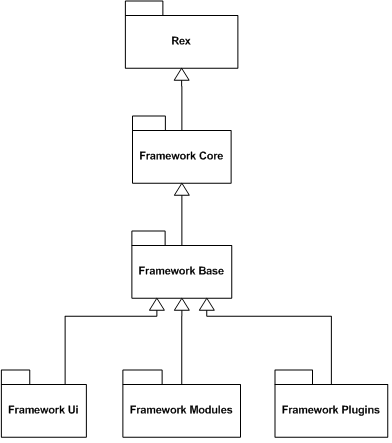
\includegraphics[height=4in,width=4in]{dev_guide_arch_packages}
\caption{Framework 3.0 package dependencies} \label{fig-arch-pkg}
\end{center}
\end{figure}

\chapter{Rex}

\par
The \textit{Rex} library is a collection of classes and modules that
may be useful to more than one project.  The most useful classes
provided by the library are documented in the following subsections.
To use the Rex library, a ruby script should require \texttt{rex}.

    \section{Assembly}

\par
When writing exploits it is often necessary to generate assembly
instructions on the fly with variable operands, such as immediate
values, registers, and so on.  To support this requirement, the Rex
library provides classes under the \texttt{Rex::Arch} namespace that
implement architecture-dependent opcode generation routines as well
as other architecture-specific methods, like integer packing.

        \subsection{Integer packing}

\par
Packing an integer depends on the byte-ordering of the target
architecture, whether it be big endian or little endian.  The
\texttt{Rex::Arch.pack\_addr} method supports packing an integer
using the supplied architecture type (\texttt{ARCH\_XXX}) as an
indication of which byte-ordering to use.

        \subsection{Stack pointer adjustment}

\par
Some exploits require the stack pointer be adjusted prior to the
execution of a payload that modifies the stack in order to prevent
corruption of the payload itself.  To support this, the
\texttt{Rex::Arch.adjust\_stack\_pointer} method provides a way to
generate the opcodes that lead to adjusting the stack pointer of a
given architecture by the supplied adjustment value.  The adjustment
value can be positive or negative.

        \subsection{Architecture-specific opcode generation}

\par
Each architecture that currently has support for dynamically
generating instruction opcodes has a class under the
\texttt{Rex::Arch} namespace, such as \texttt{Rex::Arch::X86}.  The
X86 class has support for generating \texttt{jmp}, \texttt{call},
\texttt{push}, \texttt{mov}, \texttt{add}, and \texttt{sub}
instructions.

    \section{Encoding}

\par
Encoding buffers using algorithms like XOR can sometimes be useful
outside the context of an exploit.  For that reason, the Rex library
provides a basic set of classes that implement different types of
XOR encoders, such as variable length key XOR encoders and additive
feedback XOR encoders.  These classes are used by the framework to
implement different types of basic encoders that can be used by
encoder modules.  The classes for encoding buffers can be found in
the \texttt{Rex::Encoding} namespace.

    \section{Exploitation}

\par
Often times vulnerabilities will share a common attack vector or
will require a specific order of operations in order to achieve the
end-goal of code execution.  To assist in that matter, the Rex
library has a set of classes that implement some of the common
necessities that exploits may have.

        \subsection{Egghunter}

\par
In some cases the exploitation of a vulnerability may be limited by
the amount of payload space that exists in the area of the overflow.
This can sometimes prevent normal methods of exploitation from being
possible due to the inability to fit a standard payload in the
amount of room that is available.  To solve this problem, an exploit
writer can make use of an \textit{egghunting} payload that searches
the target process' address space for an egg that is prefixed to a
larger payload.  This requires that an attacker have the ability to
stick the larger payload somewhere else in memory prior to
exploitation.  In the event that an egghunter is necessary, the
\texttt{Rex::Exploitation::Egghunter} class can be used.

        \subsection{SEH record generation}

\par
One attack vector that is particularly common on the Windows
platform is what is referred to as an SEH overwrite.  When this
occurs, an SEH registration record is overwritten on the stack with
user-controlled data.  To leverage this, the handler address of the
registration record is pointed to an address that will either
directly or indirectly lead to control of execution flow.  To make
this work, most attackers will point the handler address at the
location of a \texttt{pop/pop/ret} instruction set somewhere in the
address space. This action returns four bytes before the location of
the handler address on the stack.  In most cases, attackers will set
two of the four bytes to be equivalent a short jump instruction that
hops over the handler address and into the payload controlled by the
attacker.

\par
While the common approach works fine, there is plenty of room for
improvement.  The \texttt{Rex::Exploitation::Seh} class provides
support for generating the normal (static) SEH registration record
via the \texttt{generate\_static\_seh\_record} method.  However, it
also supports the generation of a dynamic registration record that
has a random short jump length and random padding between the end of
the registration record and the actual payload.  This can be used to
make the exploit harder to signature in an IDS environment.  The
generation of a dynamic registration record is provided by
\texttt{generate\_dynamic\_seh\_record}.  Both methods are wrapped
by the \texttt{generate\_seh\_record} method that decides which of
the two methods to use based on evasion levels.

    \section{Jobs}
    \label{rex-jobs}

\par
In some cases it is helpful to break certain tasks down into the
concept of jobs.  Jobs are simply defined as finite workitems that
have a specific task.  Using this definition, the Rex library
provides a class named \texttt{Rex::JobContainer} that exposes an
interface for coordinating various finite tasks in a centralized
manner. New jobs can be added to the job container by calling the
\texttt{add\_job} method.  Once added, a job can be started by
issuing a call to the \texttt{start\_job} method.  At any time, a
job can be stopped by calling the \texttt{stop\_job} which will also
remove the job by calling the \texttt{remove\_job} method.

\par
For more information about the usage of these API routines, please
refer to the auto-generated documentation on Metasploit website.

    \section{Logging}

\par
The Rex library provides support for the basic logging of strings to
arbitrary log sinks, such as a flat file or a database.  The logging
interface is exposed to programmers through a set of
globally-defined methods: \texttt{dlog}, \texttt{ilog},
\texttt{wlog}, \texttt{elog}, and \texttt{rlog}.  These methods
represent debug logging, information logging, warning logging, error
logging, and raw logging respectively.  Each method can be passed a
log message, a log source (the name of the component or package that
the message came from), and a log level which is a number between
zero and three.  Log sources can be registered on the fly by
\texttt{register\_log\_source} and their log level can be set by
\texttt{set\_log\_level}.

\par
The log levels are meant to make it easy to hide verbose log
messages when they are not necessary.  The use of the three log
levels is defined below:

        \subsection{LEV\_0 - Default}

This log level is the default log level if none is specified.  It
should be used when a log message should always be displayed when
logging is enabled. Very few log messages should occur at this level
aside from necessary information logging and error/warning logging.
Debug logging at level zero is not advised.

        \subsection{LEV\_1 - Extra}

This log level should be used when extra information may be needed
to understand the cause of an error or warning message or to get
debugging information that might give clues as to why something is
happening.  This log level should be used only when information may
be useful to understanding the behavior of something at a basic
level.  This log level should not be used in an exhaustively verbose
fashion.

        \subsection{LEV\_2 - Verbose}

This log level should be used when verbose information may be needed
to analyze the behavior of the framework.  This should be the
default log level for all detailed information not falling into
LEV\_0 or LEV\_1. It is recommended that this log level be used by
default if you are unsure.

        \subsection{LEV\_3 - Insanity}

This log level should contain very verbose information about the
behavior of the framework, such as detailed information about variable
states at certain phases including, but not limited to, loop iterations,
function calls, and so on.  This log level will rarely be displayed,
but when it is the information provided should make it easy to analyze
any problem.

    \section{Opcode Database}

\par
The rex library provides a class that makes it possible to interact
with the Metasploit opcode database in a programmatic fashion.  The
class that provides this feature can be found in
\texttt{Rex::Exploitation::OpcodeDb::Client}.  To learn more about
interacting with the opcode database using this interface, please
refer to the auto-generated documentation on the Metasploit website.

    \section{Post-exploitation}

\par
The rex library provides client-side implementations for some
advanced post-exploitation suites, such as DispatchNinja and
Meterpreter. These two post-exploitation client interfaces are
designed to be usable outside of the context of an exploit.  The
\texttt{Rex::Post} namespace provides a set of classes at its root
that are meant to act as a generalized interface to remote systems
via the post-exploitation clients, if supported.  These classes
allow programmers to write automated tools that can operate upon
remote machines in a platform-independent manner.  While it's true
that platforms may lack analogous feature sets for some actions, the
majority of the common set of actions will have functional
equivalents.

    \section{Protocols}

\par
Support for some of the more common protocols, such as HTTP and SMB,
is included in the rex library to help with the development of
protocol-specific exploits and to allow for ease of use in other
projects.  Each protocol implementation exists under the
\texttt{Rex::Proto} namespace.

        \subsection{DCERC}

\par
The rex library supports a fairly robust implementation of a
porition of the DCERPC feature-set and includes support for doing
evasive actions such as multi-context bind and packet fragmentation.
The classes that support the DCERPC client interface can be found in
the \texttt{Rex::Proto::DCERPC} namespace.

        \subsection{HTTP}

\par
Minimal support for an HTTP client and server is provided in the rex
library.  While similar protocol class implementations are provided
both in webrick and in other areas of the ruby default standard
library set, it was deemed that the current implementations were not
well suited for general purpose use due to the existence of blocking
request parsing and other such things.  The rex-provided HTTP
library also provides classes for parsing HTTP requests and
responses.  The HTTP protocol classes can be found under the
\texttt{Rex::Proto::Http} namespace.

        \subsection{SMB}

\par
Robust support for the SMB protocol is provided by the classes in
the \texttt{Rex::Proto::SMB} namespace.  These classes support
connecting to SMB servers and performing logins as well as other
SMB-exposed actions like transacting a named pipe and performing
other specific commands.  The SMB classes are particularly useful
for exploits that require communicating with an SMB server.

    \section{Services}

\par
One of the limitations identified in the 2.x branch of the framework
was that it was not possible to share listeners on the local machine
when attempting to perform two different exploits that both needed
to listen on the same port.  To solve this problem, the 3.0 version
of the framework provides the concept of \textit{services} which are
registered listeners that are initialized once and then subsequently
shared by future requests to allocate the same service.  This makes
it possible to do things like have two exploits waiting for an HTTP
request on port 80 without having any sort of specific conflicts.
This is especially useful because it makes it possible to not have
to worry about firewall restrictions on outbound ports that would
normally only permit connections to port 80, thus making it possible
to try multiple client-side exploits against a host with all the
different exploit instances listening on the same port for requests.

\par
Aside from the sharing of HTTP-like services, the service subsystem
also provides a way to relay connections from a local TCP port to an
already existing stream.  This support is offered through the
\texttt{Rex::Services::LocalRelay} class.

    \section{Sockets}

\par
One of the most important features of the rex library is the set of
classes that wrapper sockets.  The socket subsystem provides an
interface for creating sockets of a given protocol using what is
referred to as a \texttt{Comm} factory class.  The purpose of the
Comm factory class is to make the underlying transport and classes
used to establish the connection for a given socket opaque.  This
makes it possible for socket connections to be established using the
local socket facilities as well as by using some sort of tunneled
socket proxying system as is the case with Meterpreter connection
pivoting.

\par
Sockets are created using the socket \texttt{Parameter} class which
is initialized either directly or through the use of a hash.  The
hash initialization of the Parameters class is much the same as
perl's socket initialization.  The hash attributes supported by the
Parameter class are documented in the constructor of the Parameter
class.

\par
There are a few different ways to create sockets.  The first way is
to simply call \texttt{Rex::Socket.create} with a hash that will be
used to create a socket of the appropriate type using the supplied
or default Comm factory class.  A second approach that can be used
is to call the \texttt{Rex::Socket::create\_param} method which
takes an initialized Parameter instance as an argument.  The
remaining approaches involve using protocol-specific factory
methods, such as \texttt{create\_tcp}, \texttt{create\_tcp\_server},
and \texttt{create\_udp}.  All three of these methods take a hash as
a parameter that is translated into a Parameter instance and passed
on for actual creation.

\par
All sockets have five major attributes that are shared in common,
though some may not always be initialized.  The first attributes
provide information about the remote host and port and are exposed
through the \texttt{peerhost} and \texttt{peerport} attributes,
respectively.  The second attributes provide information the local
host and port and are exposed through the \texttt{localhost} and
\texttt{localport} attributes, respectively.  Finally, every socket
has a hash of contextual information that was used during it's
creation which is exposed through the \texttt{context} attribute.
While most exploits will have an empty hash, some exploits may have
a hash that contains state information that can be used to track the
originator of the socket.  The framework makes use of this feature
to associate sockets with framework, exploit, and payload instances.

        \subsection{Comm classes}

\par
The \texttt{Comm} interface used in the library has one simple
method called \texttt{create} which takes a \texttt{Parameter}
instance.  The purpose of this factory approach is to provide a
location and transport independent way of creating compatible socket
object instances using a generalized factory method.  For
connections being established directly from the local box, the
\texttt{Rex::Socket::Comm::Local} class is used.  For connections be
established through another machine, a medium specific Comm factory
is used, such as the Meterpreter Comm class.

\par
The \texttt{Comm} interface also supports registered event
notification handlers for when certain things occur, like prior to
and after the creation of a new socket.  This can be used by
external projects to augment the feature set of a socket or to
change its default behavior.

        \subsection{TCP sockets}

\par
TCP sockets in the Rex library are implemented as a mixin,
\texttt{Rex::Socket::Tcp}, that extends the built-in ruby Socket
base class when the local Comm factory is used.  This mixin also
includes the \texttt{Rex::IO::Stream} and \texttt{Rex::Socket}
mixins.  For TCP servers, the \texttt{Rex::Socket::TcpServer} class
should be used.

        \subsection{SSL sockets}

\par
SSL sockets are implemented on top of the normal Rex TCP socket
mixin and makes use of the OpenSSL Ruby support.  The module used
for SSL TCP sockets is \texttt{Rex::Socket::SslTcp}.

        \subsection{Switch board routing table}

\par
One of the advancements in the 3.0 version of the framework is the
concept of a local routing table that controls which Comm factory is
used for a particular route.  The reason this is useful is for
scenarios where a box is compromised that straddles an internal
network that can't be directly reached.  By adjusting the switch
board routing table to point the local subnet through a Meterpreter
Comm running on the host that straddles the network, it is possible
to force the socket library to automatically use the Meterpreter
Comm factory when anything tries to communicate with hosts on the
local subnet.  This support is implemented through the
\texttt{Rex::Socket::SwitchBoard} class.

        \subsection{Subnet walking}

\par
The \texttt{Rex::Socket::SubnetWalker} class provides a way of
enumerating all the IP addresses in a subnet as described by a
subnet address and a netmask.

    \section{Synchronization}

\par
Due to the use of multi-threading, the Rex library provides extra
classes that don't exist by default in the Ruby standard library.
These classes provide extra synchronization primitives.

        \subsection{Notification events}

\par
While Ruby does have the concept of a \texttt{ConditionVariable}, it
lacks the complete concept of notification events.  Notification
events are used extensively on platforms like Windows.  These events
can be waited on and signaled, either permanently or temporarily.
Please refer to Microsoft's online documentation for more
information. This support is provided by the
\texttt{Rex::Sync::Event} class.

        \subsection{Reader/Writer locks}

\par
A common threading primitive is the reader/writer lock.
Reader/writer locks are used to make it possible for multiple
threads to be reading a resource concurrently while only permitting
exclusive access to one thread when write operations are necessary.
This primitive is especially useful for resources that are not
updated very often as it can drastically reduce lock contentions.
While it may be overkill to have such a synchronization primitive in
the library, it's still cool.

\par
The reader/writer lock implementation is provided by the
\texttt{Rex::ReadWriteLock} class.  To lock the resource for read,
the \texttt{lock\_read} method can be used.  To lock the resource
for write access, the \texttt{lock\_write} method can be used.

        \subsection{Reference counting}

\par
In some cases it is necessary to reference count an instance in a
synchronized fashion so that it is not cleaned up or destroyed until
the last reference is gone.  For this purpose, the \texttt{Rex::Ref}
class can be used with the \texttt{refinit} method for initializing
references to 1 and the \texttt{ref} and \texttt{deref} methods that
do what their names imply.  When the reference count drops to zero,
the \texttt{cleanup} method is called on the object instance to give
it a chance to restore things back to normal in a manner similar to
a destructor.

        \subsection{Thread-safe operations}

\par
Some of the built-in functions in Ruby are not thread safe in that
they can block other ruby threads from being scheduled in certain
conditions.  To solve this problem, the functions that have issues
have been wrappered with implementations that ensure that not all
ruby threads will block.  The specific methods that required change
were \texttt{select} and \texttt{sleep}.

    \section{Ui}

\par
The Rex library provides a set of helper classes that may be useful
to certain user interface mediums.  These classes are not included
by default when requiring \texttt{rex}, so a programmer must be sure
to require \texttt{rex/ui} to get the classes described in this
section.  At the time of this writing, the only user interface
medium that has any concrete classes defined is the text, which is
synonymous with the console, user interface medium.

        \subsection{Text}

\par
The text user interface medium provides classes that allow a
programmer to interact with a terminal's input and output handles.
It also provides classes for simulating a pseudo-command shell in as
robust as manner as possible.

            \subsubsection{Input}

\par
The \texttt{Rex::Ui::Text::Input} class acts as a base class for
more specific user input mediums.  The base class interface provides
a basic set of methods for reading input from the user
(\texttt{gets}), checking if standard input has closed
(\texttt{eof?}), and others.  There are currently two classes that
extend the base class.  The first is
\texttt{Rex::Ui::Text::Input::Stdio}.  This class simply makes use
of the \texttt{\$stdin} globally scoped variable in Ruby.  This is
the most basic form of acquiring user input.  The second class is
\texttt{Rex::Ui::Text::Input::Readline} which interacts with the
user through the readline library.  If no readline installation is
present, the class will not be usable.  These two classes can be
used by the shell classes described later in this subsection.

            \subsubsection{Output}

The \texttt{Rex::Ui::Text::Output} class implements the more
generalized \texttt{Rex::Ui::Output} abstract interface.  The
purpose of the class is to define a set of functions that can be
used to provide the user with output.  There are currently two
classes that implement the textual output interface.  The first is
\texttt{Rex::Ui::Text::Output::Buffer}.  This output medium
serializes printed text to a buffer that can be retrieved via the
instance's \texttt{buf} attribute.  The second class is
\texttt{Rex::Ui::Text::Output::Stdio}.  This class is the complement
to the stdio input class and simply uses the \texttt{\$stdout}
global variable to supply the user's terminal with output.

            \subsubsection{Shell}

\par
The \texttt{Rex::Ui::Text::Shell} class provides a simple
pseudo-shell base class that can be used to implement an interactive
prompting shell with a user.  The class is instantiated by passing a
prompt string and a prompt character (which defaults to \verb#>#) to
the constructor.  By default, the shell's input and output class
instances are initialized to instances of the
\texttt{Rex::Ui::Text::Input::Stdio} and
\texttt{Rex::Ui::Text::Output::Stdio}, respectively.  To change the
input and output class instances, a call can be made to the
\texttt{init\_ui} method.

\par
To use the shell, a call must be made to the shell instance's
\texttt{run} method.  This method accepts either a block context,
which will be passed line-based input strings, or will operate in a
callback mode where a call is made to the \texttt{run\_single}
method on the shell instance.  If the second method is used, the
class is intended to be overridden with a custom implementation of
the \texttt{run\_single} method.

            \subsubsection{Dispatcher Shell}

\par
The \texttt{Rex::Ui::Text::DispatcherShell} class extends the
\texttt{Rex::Ui::Text::Shell} class by introducing the concept of a
generalized command dispatcher interface.  The dispatcher shell
works by overriding the \texttt{run\_single} method.  Unlike the
base shell class, the dispatcher shell provides a mechanism by which
command dispatchers can be registered for processing input text in a
normalized fashion.  All command dispatchers should include the
\texttt{Rex::Ui::Text::DispatcherShell::CommandDispatcher} mixin
which provides a set of helper methods, mainly dealing without
wrappering the output of text.

\par
The registration of a command dispatcher is accomplished by calling
either \texttt{enstack\_dispatcher} or \texttt{append\_dispatcher}.
The \texttt{enstack\_dispatcher} front inserts the supplied command
dispatcher instance so that it will have the first opportunity to
process commands.  The \texttt{append\_dispatcher} method inserts
the supplied command dispatcher instance at the end of the list.  To
remove command dispatchers, the complementary methods
\texttt{destack\_dispatcher} and \texttt{remove\_dispatcher} can be
used.

\par
When a line of input arrives, the base shell class calls the
overridden \texttt{run\_single} method which breaks the input string
down into an array of arguments as delimited by normal shell
characters.  The first argument in the string is then evaluated in
relation to all of the registered command dispatchers by checking to
see if any of them implement a method called \texttt{cmd\_<arg 0>}.
If they do, the dispatcher shell calls the method and passes it the
parsed argument array.

\par
In order to make it possible to automatically generate a help menu
for all registered command dispatchers, each command dispatcher
should implement a method named \texttt{commands} which should
return a hash that associates commands with a description of the
operation they perform.

            \subsubsection{Table}

\par
The \texttt{Rex::Ui::Text::Table} class can be used to format data
in the form of a table with a header, columns, and rows.  For more
information on using the table class, please refer to the
auto-generated API documentation on the Metasploit website.

            \subsubsection{Subscribers}

\par
The Rex library supports creating classes that are designed to
subscribe to input and output interfaces via the
\texttt{Rex::Ui::Subscriber} interface.  This mixin provides a
method called \texttt{init\_ui} which can be passed an input and
output class instance.  These instances should implement the
\texttt{Rex::Ui::Text::Input} and \texttt{Rex::Ui::Output}
interfaces, respectively.  Once \texttt{init\_ui} has been called,
subsequent calls to methods like \texttt{print\_line} will be passed
down into the initialized output class instance.  If no class
instance has been defined, the call will be ignored.  This makes it
possible to provide a way by which classes can interact with the
user interface only when desired.  To disable user interface
interaction, a call can be made to \texttt{reset\_ui} which will
disable future input and output classes for the class.

\chapter{Framework Core}

\par
The framework core implements the set of classes that provide an
interface to framework modules and plugins.  The core portion of the
framework is designed by used in an instance-based approach.  This
means that the entire framework state can be contained within one
class instance thereby allowing programmers to have multiple
concurrent and separate framework instances in use at the same time
rather than forcing everything to share one singleton instance.

\par
The current major version of the framework core can be accessed
through \texttt{Msf::Framework::Major} and the minor version can be
accessed through \texttt{Msf::Framework::Minor}.  A combined version
of these two version numbers can be accessed through
\texttt{Msf::Framework::Version} or \texttt{framework.version} on an
instance level.  The current revision of the framework core
interface can be accessed through
\\\texttt{Msf::Framework::Revision}.

\par
The framework core is accessed through an instance of the
\texttt{Msf::Framework} class.  Creating an instance of the
framework is illustrated in figure \ref{fig-code-framework-create}.

\begin{figure}[h]
\begin{verbatim}

framework = Msf::Framework.new
\end{verbatim}
\caption{Creating an instance of the framework}
\label{fig-code-framework-create}
\end{figure}

\par
The framework instance itself is nothing more than a way of
connecting the different critical subsystems of the framework core,
such as module management, session management, event dispatching,
and so on.  The manner of using these subsystems will be described
in the following subsections.  To use the framework core library, a
ruby script should require \texttt{msf/core}.

    \section{DataStore}

\par
Each framework instance has an instance of the
\texttt{Msf::DataStore} class that can be accessed via
\texttt{framework.datastore}.  The purpose of the datastore in the
3.0 version of the framework is to act as a replacement for the
concept of the environment in the 2.x branch.  The datastore is
simply a hash of values that may be used either by modules or by the
framework itself to reference programmer or user controlled values.
Interacting with the datastore is illustrated in figure
\ref{fig-code-framework-datastore}.

\begin{figure}[h]
\begin{verbatim}

framework.datastore['foo'] = 'bar'

if (framework.datastore['foo'] == 'bar')
    puts "'foo' is 'bar'"
end
\end{verbatim}
\caption{Creating an instance of the framework}
\label{fig-code-framework-datastore}
\end{figure}

\par
Modules will inherit values from the framework's global datastore if
they are not found in the module's localized datastore.  This aspect
will be discussed in more detail in chapter \ref{framework-modules}.

    \section{Event Notifications}

\par
One of the major goals with the 3.0 version of the framework was to
provide developers with a useful event notification system that
would allow them to perform arbitrary actions when certain framework
events occurred.  To support this, each framework instance can have
event handlers registered through the \texttt{framework.events}
attribute which is an instance of the \texttt{Msf::EventDispatcher}
class.

\par
The \texttt{EventDispatcher} class supports registering event
handlers for a few basic different categories.  These categories
will be discussed individually.  One of the nice aspects of the
event-driven framework is that modules can automatically indicate
their interest in being registered for event handler notifications
by simply implementing the event subscriber mixins described below.
When a module is loaded into the framework, it will automatically
detect that it includes one or more of the subscriber interfaces and
automatically register the module with the appropriate event
notifiers.  This makes it possible for modules to take certain
actions when specific events occur.

        \subsection{Exploit events}

\par
Event subscribers can be registered to be notified when events
regarding exploitation occur.  To register an exploit event
subscriber, a call should be made to
\texttt{framework.events.register\_exploit\_subscriber}.  This
method should be passed an instance of an object that includes the
\texttt{Msf::ExploitEvent} mixin.  The type of event that this
subscriber will be notified of is when an exploit succeeds.  In the
event that an exploit succeeds, the subscriber's
\texttt{on\_exploit\_success} method will be called with the exploit
instance that succeeded and the session instance that it created.

\par
To remove an event subscriber, a call should be made to\\
\texttt{framework.events.remove\_exploit\_subscriber} passing the
object instance that was used to add the subscriber in the first
place.

        \subsection{General framework events}

\par
To receive event notifications about internal framework events, a
general event subscriber can be registered through the
\texttt{framework.events.register\_general\_subscriber} method.
This method takes an instance of an object that includes the
\texttt{Msf::GeneralEventSubscriber} mixin.  When a module is loaded
into the framework instance, the \texttt{on\_module\_load\_proc}
will be called if it is non-nil and will be passed the reference
name and class associated with the newly loaded module. When a
module instance is created, the \texttt{on\_module\_created\_proc}
will be called if it's non-nil and will be passed the newly created
module instance.

\par
To remove an event subscriber, a call should be made to\\
\texttt{framework.events.remove\_general\_subscriber} passing the
object instance that was used to add the subscriber in the first
place.

        \subsection{Recon events}

\par
To receive notifications about reconnaissance events, such as when a
new host or service is detected, a recon event subscriber can be
registered through the
\texttt{framework.events.add\_recon\_subscriber} method.  This
method takes an instance of an object that implements one or both of
the \texttt{Msf::ReconEvent::HostSubscriber} or
\texttt{Msf::ReconEvent::ServiceSubscriber} mixins.  When a new host
is detected or an attribute of a host has changed, a call will be
made to the event subscriber's \texttt{on\_host\_changed} method
assuming it implements the \texttt{Msf::ReconEvent::HostSubscriber}
mixin.  When a new service is detected or an attribute of a service
has changed, a call will be made to the event subscriber's
\texttt{on\_service\_changed} method assuming it implements the
\texttt{Msf::ReconEvent::ServiceSubscriber} mixin.

\par
To remove an event subscriber, a call should be made to\\
\texttt{framework.events.remove\_recon\_subscriber} passing the
object instance that was used to add the subscriber in the first
place.

        \subsection{Session events}

\par
To receive notifications about events pertaining to sessions, a
session event subscriber can be registered through the
\texttt{framework.events.add\_session\_subscriber} method.  This
method takes an instance of an object that implements the
\texttt{Msf::SessionEvent} mixin.  When a new session is opened, the
framework will call into the subscriber's \texttt{on\_session\_open}
method with the session instance that has just been opened as the
first argument.  When a session terminates, the framework will call
into the subscriber's \texttt{on\_session\_close} method with the
session instance that is being closed.

\par
To remove an event subscriber, a call should be made to\\
\texttt{framework.events.remove\_session\_subscriber} passing the
object instance that was used to add the subscriber in the first
place.

    \section{Framework Managers}

\par
The framework core itself is composed of a few different managers
that are responsible for some of the basic aspects of the framework,
such as module and plugin management.

        \subsection{Module management}

\par
The module management aspect of the framework is one of its most
integral parts.  The \texttt{Msf::ModuleManager} class is
responsible for providing the interface for loading modules and for
acting as a factory for module instance creation.  The module
manager itself can be accessed through the
\texttt{framework.modules} attribute.  The loading of modules is
accomplished by adding a search path to the module manager by making
a call to the \texttt{add\_module\_path} method.  This method will
automatically load all of the modules found within the supplied
directory\footnote{The module path must conform to the standard
module directory layout, with the base directory structure appearing
similar to the \texttt{modules} sub-directory in the framework
distribution}.

\par
Modules are symbolically identified by what is referred to as a
\textit{reference name}.  The reference name takes a form that is
similar to a directory path and is partially controlled by the
filesystem path that the module is loaded from.  An example of a
reference name would be an exploit labeled
\texttt{windows/ftp/wsftpd}.  This would mean that the exploit was
loaded from \texttt{exploits/windows/ftp/wsftpd.rb}.  It is
important to note that module's must retain a namespace hierarchy
that mirrors the path in which they are located.  For instance, the
example described previously would have the class declared as
\texttt{Msf::Exploits::Windows::Ftp::Wsftpd}.  This is necessary so
that the framework's module manager knows what namespace to look in
to see what class was added after loading the file.  The reference
name of a module can be accessed through the \texttt{refname}
attribute on both the class of the module and its instances.

\par
In order to help solve the potential for module name ambiguities
across module types, modules can also be referenced to by what is
called a \textit{full reference name}.  This name is the same as the
reference name of the module but is prefixed with the module's type.
For instance, the exploit \texttt{windows/ftp/wsftpd} would become
\texttt{exploit/windows/ftp/wsftpd}.  The full reference named can
be accessed through the \texttt{fullname} attribute on both the
class of the module and its instances.

\par
In order to make the module manager easy to use, each different
module type is broken down into a more basic class called a module
set which is implemented by the \texttt{Msf::ModuleSet} class.  The
purpose of a module set is to act as a localized factory for each
different module type (exploit, encoder, nop, etc).  Each
type-specific module set can be accessed through either
\texttt{framework.type} or \texttt{framework.modules.type}.  For
example, if one wanted to enumerate exploit modules, they would use
the \texttt{framework.exploits} method to get access to the exploit
module set.

\par
Module sets are implemented in the form of a hash that associates
the reference names of modules with their underlying classes.  To
create an instance of a module, a call is made to the module set's
\texttt{create} method passing the reference name of the module that
should be instantiated.  For example, to create an instance of an
exploit named \texttt{windows/ftp/wsftpd}, a call would be made as
shown in figure \ref{fig-code-framework-modcreate}

\begin{figure}[h]
\begin{verbatim}
framework.exploits.create('windows/ftp/wsftpd')
\end{verbatim}
\caption{Creating an instance of a framework module}
\label{fig-code-framework-modcreate}
\end{figure}

\par
The table shown in figure \ref{fig-table-modulsets} shows the
relation between module types and framework module set accessors.

\begin{figure}[h]
\begin{center}
\begin{tabular}{|l|l|}
\hline
\textbf{Module Type} & \textbf{Accessor} \\
\hline
MODULE\_ENCODER & framework.encoders \\
MODULE\_EXPLOIT & framework.exploits \\
MODULE\_NOP & framework.nops \\
MODULE\_RECON & framework.recon \\
MODULE\_PAYLOAD & framework.payloads \\
\hline
\end{tabular}
\caption{Module types and their framework accessors}
\label{fig-table-modulsets}
\end{center}
\end{figure}

\par
To reload the contents of a module, a call can be issued to
\texttt{reload\_module} passing the module instance that should be
reloaded.  This will lead to the framework re-reading the contents
of the module's underlying file path and automatically creating a
new instance of the module.

        \subsection{Plugin management}

\par
One of the new features in the 3.0 version of the framework is the
concept of framework plugins.  Unlike modules, framework plugins are
meant to add features to the framework or to change the behavior of
existing aspects of the framework.  Plugins have a very loose
definition in terms of the scope in which they can operate.  For
instance, a plugin could add an entirely new module type for use by
the framework.  Alternatively, a plugin could add commands to the
existing user interfaces that interact with the framework.  A plugin
could also register custom event subscribers for doing things like
automatically causing Meterpreter to list the contents of a
computer's C drive when a new Meterpreter session is created.  The
possibilities, as they say, are endless.

\par
The plugin manager can be accessed through the
\texttt{framework.plugins} accessor which is an instance of the
\texttt{Msf::PluginManager} class. To load a plugin, a call can be
made to \texttt{framework.plugins.load} with the path of the plugin
that is to be loaded.  Optionally, a second parameter can be passed
to the \texttt{load} method that is a hash of option parameters that
may be useful to the plugin, such as \texttt{LocalInput} and
\texttt{LocalOutput} handles for use with printing strings to the
screen for whatever medium is currently being used.  The table shown
in figure \ref{fig-table-plugin-hash} shows the pre-defined hash
elements that can be passed in the option hash.

\begin{figure}[h]
\begin{center}
\begin{tabular}{|l|p{3.5in}|}
\hline
\textbf{Hash Element} & \textbf{Description} \\
\hline
LocalInput & The local input class instance which implements the \texttt{Rex::Ui::Text::Input} interface. \\
\hline
LocalOutput & The local input class instance which implements the \texttt{Rex::Ui::Output} interface. \\
\hline
ConsoleDriver & The console driver instance of \texttt{Msf::Ui::Console::Driver}. \\
\hline
WebDriver & The console driver instance of \texttt{Msf::Ui::Web::Driver}. \\
\hline
\end{tabular}
\caption{Plugin optional constructor hash elements}
\label{fig-table-plugin-hash}
\end{center}
\end{figure}

\par
All plugins are reference counted.  This is to make it possible to
implement singleton plugins that could possibly be loaded more than
once but will only have one underlying instance.  The reference
count to an instance of a plugin is automatically incremented each
time \texttt{load} is called on it.

\par
To unload a framework plugin, a call can be made to
\texttt{framework.plugins.unload} passing the instance of the plugin
previously loaded as the first parameter.  Since all plugins are
reference counted, a plugin will not actually be unloaded until its
reference count drops to zero.

\par
For more detail on the implementation of framework plugins, please
see chapter \ref{framework-plugins}.

        \subsection{Recon management}

\par
The reconnaissance manager is used to provide an interface for
reporting information about hosts, services, and other
reconnaissance entities.  These reports are tracked internally by
the recon manager which is implemented by the
\texttt{Msf::ReconManager} class.  The recon manager can be accessed
through the \texttt{framework.reconmgr} accessor.

\par
This area of the framework is currently undergoing design review and
therefore does not have any documentation at this time.

        \subsection{Session management}

\par
The session manager is used to track sessions created from within a
framework instance as the result of an exploit succeeding.  The
purpose of sessions is to expose features to a programmer that allow
it to be interacted with.  For instance, a command shell session
allows programmers to send commands and read responses to those
commands through a well-defined API.  For more information on
sessions and how they can be interacted with, please see chapter
\ref{framework-sessions}.  The session manager itself can be
accessed through the \texttt{framework.sessions} accessor and is an
instance of the \texttt{Msf::SessionManager} class.

\par
The primary purpose of the session manager is to provide an
interface for registering new sessions and assigning them a unique
session identifier as well as allowing sessions to be deregistered
when they are destroyed.  The registering of sessions with the
framework session manager is accomplished by making a call into the
\texttt{framework.sessions.register} method which takes an instance
of a session as its argument.  This method will assign the session a
unique session identifier and add it to the managed hash of
sessions.  Sessions can be enumerated by making a call into
\texttt{framework.sessions.each\_sorted} or by calling any of the
hash-compatible enumeration methods.  To obtain the session instance
associated with a particular session identifier, the
\texttt{framework.sessions.get} method can be called with the
session identifier to look up.  When a session is being destroyed, a
call must be made to \texttt{framework.sessions.deregister} passing
the instance of the session being destroyed as the first argument.

        \subsection{Job management}

\par
Each framework instance supports running various tasks in the
context of worker threads through the concept of jobs.  The job
interface can be accessed through the \texttt{framework.jobs}
accessor which is an instance of the \texttt{Rex::JobContainer}
class.  For more information on jobs, please refer to the job
explanation in the Rex documentation in section \ref{rex-jobs}.

    \section{Utility Classes}

\par
Some classes in the framework core are intended to be used to make
certain tasks simpler without being out of scope of the core aspects
of the framework.  These classes are described below.

        \subsection{Exploit driver}

\par
The \texttt{Msf::ExploitDriver} class encapsulates the task of
running an exploit module in terms of coordinating the validation of
required module options, the validation of target selection, the
generation of a selected payload, and the execution of exploit and
payload setup and cleanup.  These operations are what has to be
performed when attempting to execute an exploit.

\par
An instance of an exploit driver is initialized as described in
figure \ref{fig-code-exploit-driver}.

\begin{figure}[h]
\begin{verbatim}
driver = Msf::ExploitDriver.new(framework)

driver.payload = payload_instance
driver.exploit = exploit_instance
driver.target_idx = 0

session = driver.run
\end{verbatim}
\caption{Using the ExploitDriver class}
\label{fig-code-exploit-driver}
\end{figure}

\par
When the \texttt{run} method is called, the first step is to
validate the options required by the payload and the exploit that
have been selected.  This is done by calling the public
\texttt{validate} method on the exploit driver instance.  In the
event that options fail to validate or that a target index has not
been properly selected, an exception will be thrown to the caller.
After validation has completed, the exploit's \texttt{TARGET} data
store element is set to the selected target index.  From there, an
encoded version of the payload is generated by calling
\texttt{generate\_payload} on the exploit instance.  Once completed,
the exploit is set up by calling \texttt{setup} on the exploit
module instance and finally the actual exploit code is triggered by
calling \texttt{exploit} on the exploit module instance.

\par
Once exploitation has completed, the exploit driver calls the
\texttt{stop\_handler} method on the payload module instance and
then calls the \texttt{cleanup} method on the exploit module
instance.

\par
The exploit driver can also be instructed to run the exploit in the
context of a job.  When this is done, the underlying exploitation
operation is done in the context of a job worker thread by calling
\texttt{framework.jobs.start\_bj\_job}.  The exploit driver can be
told to use a job by setting the \texttt{use\_job} attribute to
true.

        \subsection{Encoded payload}

\par
The purpose of the \texttt{Msf::EncodedPayload} class is to
encapsulate the operation of encoding a payload with an arbitrary
set of requirements.  To generate an encoded payload, an instance of
an \texttt{Msf::EncodedPayload} class must be created by passing its
constructor an instance of a payload as well as an optional hash of
requirements that will be used during the generation phase.  This
can be accomplished by calling the class' \texttt{create} method as
shown in figure \ref{fig-code-enc-payload}.


\begin{figure}[h]
\begin{verbatim}

encoded = Msf::EncodedPayload.create(payload_instance,
    'BadChars'      => "\x0a\0xd",
    'Space'         => 400,
    'Prepend'       => "\x41\x41",
    'Append'        => "\xcc\xcc\",
    'SaveRegisters' => "edi",
    'MinNops'       => 16)
\end{verbatim}
\caption{Creating an instance of an EncodedPayload}
\label{fig-code-exploit-driver}
\end{figure}

\par
Once an encoded payload instance has been created, the next step is
to make a call to the instance's \texttt{generate} method which will
return the encoded version of the payload.  After generation has
occurred, the following attributes can be accessed on the encoded
payload instance in order to get information about the now-encoded
payload.  Figure \ref{fig-table-enc-payload} shows the attributes
and their purposes.

\begin{figure}[h]
\begin{center}
\begin{tabular}{|l|p{3.5in}|}
\hline
\textbf{Attribute} & \textbf{Description} \\
\hline
raw & The un-encoded raw payload buffer. \\
\hline
encoded & The encoded payload buffer which may be equal to raw if no encoder was used. \\
\hline
nop\_sled\_size & The size of the NOP sled prepended to the encoded payload.  Zero if no NOPs were generated. \\
\hline
nop\_sled & The NOP sled portion of the encoded payload, if any. \\
\hline encoder & The encoder module instance that was used to encode
the
payload. \\
\hline nop & The nop module instance that was used to generate the
NOP
sled, if any. \\
\hline
\end{tabular}
\caption{\texttt{Msf::EncodedPayload} instance attributes}
\label{fig-table-enc-payload}
\end{center}
\end{figure}

\par
To control the behavior of the encoded payload class, an optional
hash can be passed into the constructor.  The table in figure
\ref{fig-table-enc-payload-options} describes the options that can
be specified and the affect they have on behavior.


\begin{figure}[h]
\begin{center}
\begin{tabular}{|l|p{3.5in}|}
\hline
\textbf{Hash Element} & \textbf{Description} \\
\hline
BadChars & A string of bad characters to avoid when encoding. \\
\hline
Encoder & The name of the preferred encoder to use. \\
\hline
MinNops & The minimum number of NOPs to generate. \\
\hline
MaxNops & The maximum number of NOPs to generate. \\
\hline
Space & The amount of room left for use by the payload.  If this value is not specified, then NOP padding will not be performed and there will be no restrictions on payload size. \\
\hline
SaveRegisters & A white-space separated list of registers to save when generating the NOP sled. \\
\hline
Prepend & Raw instructions or text to prepend to the encoded payload. \\
\hline
Append & Raw instructions or text to append to the encoded payload. \\
\hline
\end{tabular}
\caption{\texttt{Msf::EncodedPayload} constructor options}
\label{fig-table-enc-payload-options}
\end{center}
\end{figure}

\chapter{Framework Base}

\par
The framework base is a library layer built on top of the framework
core that adds classes that make dealing with the framework easier.
It also provides a set of classes that could be useful to third
party development tools that don't necessarily fit within the scope
of the framework core itself.  The classes that compose the
framework base are described in the following subsections.  To use
the framework base library, a ruby script should require
\texttt{msf/base}.

    \section{Configuration}

\par
One important aspect of a managed framework installation is the
concept of persistent configuration and methods for getting
information about the structure of an installation, such as the root
directory of the installation and other types of attributes.  To
facilitate this, the framework base library provides the
\texttt{Msf::Config} class that has methods for obtaining various
installation directory paths.  It also supports the serialization of
configuration files.  The table shown in figure
\ref{fig-table-config} describes the different methods that can be
used to obtain configuration information.


\begin{figure}[h]
\begin{center}
\begin{tabular}{|l|p{3.5in}|}
\hline
\textbf{Method} & \textbf{Description} \\
\hline
install\_root & The installation's root directory. \\
\hline
config\_directory & The configuration directory (\verb#~/.msf3#). \\
\hline
module\_directory & install\_root + '/modules'. \\
\hline
plugin\_directory & install\_root + '/plugins'. \\
\hline
log\_directory & config\_directory + '/logs'. \\
\hline
session\_log\_directory & config\_directory + '/logs/sessions'. \\
\hline
user\_module\_directory & config\_directory + '/modules'. \\
\hline
data\_directory & install\_root + '/data'. \\
\hline
config\_file & config\_directory + '/config'. \\
\hline
load & Loads the contents of a configuration file and returns an instance of a \texttt{Rex::Parser::Ini} object. \\
\hline
save & Saves the supplied option hash to the configuration file supplied as \texttt{'ConfigFile'} in the options hash or the config\_file by default. \\
\hline
\end{tabular}
\caption{\texttt{Msf::Config} accessor methods}
\label{fig-table-config}
\end{center}
\end{figure}

    \section{Logging}

\par
The framework base library provides a wrapper class that can be used
to control debug logging at an administrative level by providing
methods for enabling log sources and for controlling logs that are
applied to sessions created from within a framework instance.  To
initialize logging, a call must be made to
\texttt{Msf::Logging.init} which will register the log sources
\texttt{rex}, \texttt{core}, and \texttt{base} as being directed at
\texttt{framework.log} as found in the
\texttt{Msf::Config.log\_directory}.  Individual log sources can be
subsequently enabled or disabled by making calls to
\texttt{Msf::Logging.enable\_log\_source} and
\texttt{Msf::Logging.disable\_log\_source}, respectively.  When
session logging is enabled, calls can be issued to
\texttt{start\_session\_log} and \texttt{stop\_session\_log} which
operate on a provided session instance to start or stop logging to a
session-specific log file in the
\texttt{Msf::Config.session\_log\_directory} directory.

    \section{Serialization}

\par
To make life easier for framework programmers, the framework base
library provides a class that can be used to serialize information
about modules, such as their description, options, and other
information to a uniform, human readable format.  The class that
provides this feature is the \texttt{Msf::Serializer::ReadableText}
class.  For more information, please review the auto-generated API
documentation on the Metasploit website.

    \section{Sessions}

\par
While the framework core has an abstract concept of sessions as
described through the \texttt{Msf::Session} base module, the
framework base actually provides some of the concrete
implementations.  This separation was done to eliminate
module-specific session implementations from the framework core as
the core should have no conceptual dependencies on modules that use
it.  The base library, on the other hand, is more of a facilitation
layer for subscribers of the framework.  The two sessions currently
implemented in the base library are the \texttt{CommandShell}
session and the \texttt{Meterpreter} session.

        \subsection{CommandShell}

\par
The command shell session implements the framework core \\
\texttt{Msf::Session::Provider::SingleCommandShell} interface
against a connected stream, such as a TCP connection.  For more
information about this mixin, please read chapter
\ref{framework-sessions}.

        \subsection{Meterpreter}

\par
The meterpreter session implements the
\texttt{Msf::Session::Interactive} and \\
\texttt{Msf::Session::Comm}
mixins.  This allows it to be operated through an interactive user
shell and also indicates to the framework that internet traffic can
be routed (pivoted) through the session by making use of it as a
Comm socket factory.  The session itself is merely an extension of
the \texttt{Rex::Post::Meterpreter} class which operates against a
connected stream, such as a TCP connection.

    \section{Simplified Framework}

\par
The simplified framework provides methods that make the framework
and the different module types easier to use by providing wrapper
methods that handle most of the actions that would be common to a
subscriber of the framework.  To create an instance of the
simplified framework, the \texttt{Msf::Simple::Framework.create}
method should be called along with an optional hash.  The return
value is an instance of an \texttt{Msf::Framework} class that has
been extended by the \texttt{Msf::Simple::Framework} mixin. Existing
framework instances can also be simplified by calling the
\texttt{Msf::Simple::Framework.simplify} method with the existing
framework instance as the first argument.  All module instances
created from within a simplified framework instance will
automatically be simplified by the module type-specific mixins.

\par
The creation of a simplified framework instance automatically leads
to the initialization of the \texttt{Msf::Config} class and the
\texttt{Msf::Logging} class.  Any existing configuration file is
also automatically loaded.  The default global module directory
(\texttt{Msf::Config::module\_directory}) and the user-specific
module directory (\texttt{Msf::Config::user\_module\_directory}) are
added as search paths to the framework instance which leads to the
loading of all modules within the two directories.  Finally, a
general event subscriber is registered with the framework instance
that will be called whenever module instances are created within the
framework.  This allows the simplified framework the opportunity to
simplify each created module instance.

\par
Each module type has a simplified framework module mixin that is
automatically used to extend created module instances via the
general event subscriber described above.  For example, when an
exploit module instance is created, the instance is extended by the
\texttt{Msf::Simple::Exploit} mixin.  Each different module mixin
provides a helper method or methods for driving that specific module
type's primary action or actions.  Furthermore, each module instance
has methods that can be used to save and restore module-specific
configuration elements through the \texttt{save\_config} and
\texttt{load\_config} methods.  Each module-specific mixin is
described individually below.

        \subsection{Exploit}

\par
The simplified exploit mixin provided in
\texttt{Msf::Simple::Exploit} extends each exploit module instance
with a method called \texttt{exploit\_simple}.  This method takes a
hash parameter that is used to control the exploitation of something
by creating an instance of an \texttt{Msf::ExploitDriver} class and
doing all the required initialization and configuration of the
module prior to issuing the call to the exploit driver's
\texttt{run} method.  If the operation succeeds, the return value is
a session instance.  Otherwise, an exception will be thrown or
\texttt{nil} may be returned. For more information about the hash
elements that can be passed in, please refer to the auto-generated
API documentation on the Metasploit website.

        \subsection{NOP}

\par
The simplified NOP mixin provided in \texttt{Msf::Simple::Nop}
extends each nop module instance with a method called
\texttt{generate\_simple}.  This method takes the length of the sled
generate and the hash of options that should be used for the
generation.  On success, the return value is a buffer that is
encoded using the \texttt{Msf::Simple::Buffer} class using the
format specified in the option hash as the \texttt{'Format'}
element.  If no format is specified, the raw version of the NOP sled
is returned.

        \subsection{Payload}

\par
The simplified payload mixin provided in
\texttt{Msf::Simple::Payload} extends each payload module instance
with a method called \texttt{generate\_simple}.  This method takes a
hash of options that are used to generate a payload buffer.  The
elements that can be used in the option hash can be found in the
auto-generated API documentation found on the Metasploit website. If
the operation is successful, the encoded payload buffer will be
serialized to the format supplied in the \texttt{'Format'} hash
element.  If the format is not raw, any staged payloads will also be
appended to the serialized buffer.

        \subsection{Recon}

\par
The reconnaissance interface is under design review.

\chapter{Framework Ui}

\par
The framework user interface library is used to encapsulate code
common to different user interface mediums to allow third party
development and extension of custom user interfaces separate from
those distributed with the framework itself.  Each different user
interface medium is encapsulated in an abstract \textit{driver}
class, \texttt{Msf::Ui::Driver} that is designed to have an actual
interface that is specific to the underlying user interface medium
being used.

\par
The inherited driver base class simply defines three methods that
are to be common to all user interfaces.  Those methods are
\texttt{run}, \texttt{stop}, and \texttt{cleanup}.  Their names
imply the actions that are to be performed.  Each of the currently
defined user interface mediums will be explained individually in the
following sections.  To use the framework ui library, a ruby script
should require \texttt{msf/ui}.

\chapter{Framework Modules}
\label{framework-modules}

\par
The primary purpose of the Metasploit framework is to facilitate the
development of modules that can plug into the framework core and be
shared with other existing modules.  For instance, an advanced
encoder module can be plugged into the framework and will be
automatically applied to payloads of a compatible architecture and
platform.  This makes it so there are zero code changes required due
to the fact that all modules conform to a well-defined interface
through which they can be interacted with by the framework.  As
another example, new payloads can be developed and are immediately
usable to all exploits without modification.  This eliminates the
need to copy static payload blobs into exploits as is most common
with proof of concept exploits.  This chapter is dedicated to
describing the interfaces that each module type exposes in order to
provide an understanding of what it takes to implement each module
type.

\par
At some level, all modules inherit from the module base class
provided in \texttt{Msf::Module}.  This class implements all of the
things that are common to Metasploit framework modules, such as
common accessors and attributes.  When a module is loaded into the
framework, a copy of the class that gets added is made which is what
is used for future instantiations of the module.  The copy class
then has some of its attributes set that allow the framework to look
at some of the module's information at a glance without having to
create an instance of it. This information can be accessed through a
set of class methods and attributes that are described in figure
\ref{fig-table-mod-class-methods}.

\begin{figure}[h]
\begin{center}
\begin{tabular}{|l|p{3.5in}|}
\hline
\textbf{Method} & \textbf{Description} \\
\hline
framework & The framework instance that the module is associated with. \\
\hline
type & The module's symbolic type.  One of \texttt{MODULE\_ENCODER}, \texttt{MODULE\_EXPLOIT}, \texttt{MODULE\_NOP}, \texttt{MODULE\_PAYLOAD}, or \texttt{MODULE\_RECON} \\
\hline
fullname & The complete symbolic name of the module including is string type.  For example: exploit/windows/ms03\_026 \\
\hline
rank & The module's integer rank to indicates its quality.  The rank is used by the framework when selecting which encoders, payloads, and NOP generators to use. \\
\hline
rank\_to\_s & Returns the string representation of the module's rank. \\
\hline
refname & The module's symbolic reference name.  For example: windows/ms03\_026 \\
\hline
orig\_cls & The original, non-duplicated class that was loaded for the module. \\
\hline
file\_path & The file path that the module was loaded from. \\
\hline
\end{tabular}
\caption{\texttt{Msf::Module} class methods}
\label{fig-table-mod-class-methods}
\end{center}
\end{figure}

\par
To support generic initialization, each module defines its own
custom information hash that is eventually passed to the constructor
of \texttt{Msf::Module}.  This information class is then assigned to
the instance attribute named \texttt{module\_info} and is then
processed. The parts that are common to all modules are broken down
and transformed into uniform types that can be accessed through
instance methods. The same methods that are accessible through the
module class can also be used through the class instance (as shown
in figure \ref{fig-table-mod-class-methods}).

\par
The table in figure \ref{fig-table-mod-info} shows how the common
module information hash elements are broken down into their
respective data types and the methods that can be used to access
them.

\begin{figure}[hbp]
\begin{center}
\begin{tabular}{|l|l|l|p{2.0in}|}
\hline
\textbf{Hash Element} & \textbf{Accessor} & \textbf{Type} & \textbf{Description} \\
\hline
Name & name & String & The short name of the module. \\
\hline
Alias & alias & String & An alias string for the refname of the module. \\
\hline
Description & description & String & A longer description of the module. \\
\hline
Version & version & String & The current revision of the derived module. \\
\hline
License & license & String & The license that the module has been released under. \\
\hline
Author & author & Array & An array of \texttt{Msf::Author} instances. \\
\hline
Arch & arch & Array & An array of architectures (like \texttt{ARCH\_X86}). \\
\hline
Platform & platform & PlatformList & An instance of a \texttt{Msf::PlatformList}. \\
\hline
References & references & Array & An array of \texttt{Msf::Reference} instances. \\
\hline
Options & options & OptionContainer & Options conveyed in the hash are added to the module's option container. \\
\hline
AdvancedOptions & options & OptionContainer & Options conveyed in the hash are added to the module's option container as advanced options. \\
\hline
DefaultOptions & options & OptionContainer & Previously registered options have their default value modified. \\
\hline
Privileged & privileged & Bool & Whether or not the module requires or grants privileged access. \\
\hline
Compat & compat & Hash & A hash of compatibility flags. \\
\hline
\end{tabular}
\caption{\texttt{Msf::Module} information hash accessors}
\label{fig-table-mod-info}
\end{center}
\end{figure}


\par
Some of the information hash accessors also have helper methods that
make it easier to interact with them.  For instance, the
\texttt{Arch} hash element array contained within the \texttt{arch}
attribute can be serialized to a comma separated string by calling
\texttt{arch\_to\_s}.  Architectures can also be enumerated by
calling \texttt{each\_arch} by passing it a block that accepts the
architecture as a parameter.  It is also possible to check if a
module supports an architecture by calling the \texttt{arch?} method
and passing it the architecture to check for as a parameter.  Like
architectures, platforms can be serialized to a string by calling
\texttt{platform\_to\_s}.

\par
The \texttt{Author} hash element can also be converted to a comma
separated string of authors by calling \texttt{author\_to\_s}.  The
array of \texttt{Msf::Author} instances contained within the
\texttt{author} array attribute can be enumerated by calling
\texttt{each\_author} and passing it a block that takes an author
instance as its first parameter.

\par
The \texttt{Msf::Module} class also has some helper methods that
allow users to quickly check if a module is of a specific type by
calling the \texttt{<type>?} method set.  For instance, if a caller
wished to see if a module instance was an exploit, they could call
\texttt{mod.exploit?}.

\par
Since the Rex library introduces the concept of socket communication
factories (through the \texttt{Comm} class), each module has an
attribute that can return the \texttt{Comm} instance that was used
or preferred.  By default, all modules return
\texttt{Rex::Socket::Comm::Local}.

\par
Each module has its own instance-based datastore which is an
instance of the \texttt{Msf::ModuleDataStore} class and can be
accessed through the \texttt{datastore} accessor. This mirrors the
functionality provided by the global framework datastore in that it
provides a localized variable to value association for use in
satisfying required options.  For instance, if a module requires the
\texttt{RHOST} option to be set to a value, the module's data store
must have a hash entry for \texttt{RHOST}. Alternatively, modules
are designed to be able to fall back on the framework global
datastore if their localized datastore does not have a value for a
variable being checked for. This provides a basic level of
variable/value inheritance.  In some cases, modules may wish to
share their localized copies of the datastore with other modules
without having to taint the global datastore.  This can be
accomplished by calling the \texttt{share\_datastore} method on a
module instance and passing it a data store instance as the first
argument.

\par
Finally, framework modules are designed to be able to indicate their
relative compatibilities with other modules.  For instance, an
exploit may wish to indicate that it is incompatible with a specific
class of payload connection mediums.  This is accomplished through
the \texttt{Compat} information hash element.  After the
compatibility layer has been initialized, calls can be made to a
module's \texttt{compatible?} method by passing another module
instance as the argument.  If the supplied module instance is
compatible with the instance that's being checked against, then true
is returned.

\par
This basic interface provides a generalized view into the behavior
and expectations of framework modules.  However, all module types
have well-defined interfaces for dealing with the actions that they
are meant to undertake.  These specific interfaces will be described
in the following sections.

    \section{Encoder}

\par
Encoder modules are used to generate transformed versions of raw
payloads in a way that allows them to be restored to their original
form at execution time and then subsequently executed.  To
accomplish this, most encoders will take the raw form of the payload
and run it through some kind of encoding algorithm, like bitwise
XOR.  After the encoded version is generated, a decoding stub is
prefixed to the encoded version of the payload.  This stub is
responsible for performing the inverse operation on the buffer
attached to the decoder when it executes.  After the decoder
restores the payload to its original form, it will transfer
execution to the start of the now normalized payload.

\par
To support the above described encoder model, the Metasploit
framework provides the \texttt{Msf::Encoder} class which inherits
from the \texttt{Msf::Module} base class.  All encoders must inherit
from the \texttt{Msf::Encoder} class at some level to ensure that
encoder-specific methods are included in the derived class.

\par
Like the module information hash, encoders have some specialized
information hash elements that describe information about the
encoder being used.  The information that encoder modules need to
describe are the attributes of the decoder which is conveyed through
the \texttt{Decoder} information hash element.  The \texttt{Decoder}
hash element references another hash that contains decoder specific
properties.  These are described in the table shown in figure
\ref{fig-table-encoder-hash} along with their types and module
instance accessors.

\begin{figure}[h]
\begin{center}
\begin{tabular}{|l|l|l|p{2.0in}|}
\hline
\textbf{Hash Element} & \textbf{Accessor} & \textbf{Type} & \textbf{Description} \\
\hline
Stub & decoder\_stub & String & The raw stub to be prefixed to encoded payloads. \\
\hline
KeyOffset & decoder\_key\_offset & Fixnum & The offset to the key in the decoder stub. \\
\hline
KeySize & decoder\_key\_size & Fixnum & The size of the decoder key in bytes. \\
\hline
BlockSize & decoder\_block\_size & Fixnum & The size of each encoding block in bytes. \\
\hline
KeyPack & decoder\_key\_pack & String & The byte-ordering to use when packing the key.  The default is 'V'. \\
\hline
\end{tabular}
\caption{\texttt{Msf::Encoder} \texttt{Decoder} information hash
accessors} \label{fig-table-encoder-hash}
\end{center}
\end{figure}

\par
Each of the methods described in figure \ref{fig-table-encoder-hash}
are designed to be overridable so that derived encoder classes can
dynamically choose the values returned by them rather than being
forced to initialize them in a static hash element.  The decoder
hash itself can be accessed through the \texttt{decoder\_hash}
method in case an encoder module wishes to convey non-standard
information in the hash for later reference.

\par
Perhaps of more importance that the decoder initialization vector is
how the encoding process is exposed.  The base class
\texttt{Msf::Encoder} implements an instance method named
\texttt{encode} which takes a buffer as the first argument, a string
of bad characters (or nil) as the second argument, and an optional
encoder state as the third argument.  The \texttt{encode} method
wraps the encoding process in terms of selecting a decoder key,
initializing the encoder state, and then performing the actual
encoding operation.  Once completed, the encoded buffer is returned
to the caller.  This is the primary method that the framework uses
when interacting with framework encoder modules.

        \subsection{encode}

\par
At a more detailed level, the \texttt{encode} method first creates
an instance of a \texttt{Msf::EncoderState} class if one was not
supplied as the third argument of \texttt{encode}.  The purpose of
the encoder state is to contain transient information about a
specific encoding operation in a non-global fashion.  After creating
the encoder state instance, \texttt{encode} prepends any
encoder-specific data to the raw payload that may be necessary
through the use of the \texttt{prepend\_buf} instance method on the
encoder module.  This method is intended to be overridden and used
as necessary.  By default, an empty string is returned, effectively
leaving the buffer in the same state that it was when it was passed
in.

\par
After prepending the raw buffer as necessary, the \texttt{encode}
method then selects a decoder key if the \texttt{decoder\_key\_size}
method returns a non-zero value and the encoder state currently has
a \texttt{nil} key.  This is accomplished by calling the
\texttt{find\_key} method on the encoder module which has a default
implementation that is intended to work across all encoder modules.
Once a key has been selected, the \texttt{init\_key} method is
called on the encoder state object to set the \texttt{state.key} and
\texttt{state.orig\_key} attributes.  If no key is found, a
\texttt{Msf::NoKeyError} exception is raised.

\par
The next step is to initialize some of the encoder state specific
attributes by calling the \texttt{init\_state} method on the encoder
module instance which simply stores the currently defined decoder
key offset, size, and pack as attributes of the encoder state as
conveyed through the accessor methods on the encoder module instance
itself.  The encoder state then has the string of bad characters and
the raw buffer set as attributes so that they can be contextually
referenced throughout the encoding process.

\par
With the encoder state finally initialized, the next step is to
begin the encoding process by calling the \texttt{encode\_begin}
method on the encoder module instance.  This method simply does
nothing in its default implementation, but it is designed to allow
derived encoder modules to alter the attributes of the encoder state
prior to actually starting the encoding process.  Once
\texttt{encode\_begin} returns, the \texttt{encode} method makes a
call into the \texttt{do\_encode} method by passing it the buffer,
bad characters, and initialized encoder state.  This is the method
that does the actual encoding work and could possibly be overridden
if the default implementation was not suitable for a given encoder.

\par
Once \texttt{do\_encode} completes, the \texttt{encode} method makes
a call into \texttt{encode\_end} and passes the encoder state as an
argument.  The default implementation of this method simply does
nothing, but it is provided as a means by which an encoder can hook
into the finalization of the encoding process to alter the results
that will be returned to the caller.

        \subsection{do\_encode}

\par
The \texttt{do\_encode} method is the actual workhorse of the
encoding process.  It starts by making a copy of the decoder stub by
calling the encoder module instance's \texttt{decoder\_stub} method
and passing it the encoder state as an argument.  The
\texttt{decoder\_stub} method is the only one that takes an encoder
state as an argument as some encoders may generate dynamic decoder
stubs depending on the state.

\par
After obtaining the decoder stub, the next step is to substitute the
packed version of the decoder key at whatever offset was conveyed in
the decoder information hash through the \texttt{KeyOffset} and
\texttt{KeySize} as well as the \texttt{KeyPack}.  These attributes
are gotten through the encoder state's attributes since it's
possible that a derived encoder may wish to alter their values to be
non-static between iterations of the encoding process.

\par
Finally, the actual block-based encoding occurs by simply walking
the raw buffer in block size chunks calling the
\texttt{encode\_block} method on each chunk.  This method is passed
the encoder state and the chunk to be encoded.  By default, the
\texttt{encode\_block} method simply returns the block it is passed,
but all encoders are intended to override this method to return the
encoded value of the block based on the current encoder state.

\par
After all the blocks have been encoded, the encoder state's
\texttt{encoded} attribute will contain the encoded version of each
blocked.  The \texttt{do\_encode} method then prepends the decoder
stub to the front of the encoded buffer and then checks to see if
the complete stub + encoded buffer has any bad characters.  If bad
characters are found, a \texttt{Msf::BadcharError} exception is
raised to the caller indicating what character and position the bad
character was found at in the encoded buffer.  If all goes well, the
\texttt{do\_encode} method returns true.

        \subsection{Helper methods}

\par
Internal the encoder module class are some instance helper methods
that can be used by derived classes to make things easier.  For
instance, the encoder module base class has a method called
\texttt{has\_badchars?} that can be used to check to see if the
supplied buffer has any of the supplied bad characters.  If it does,
the index of the first bad character found is returned.  Otherwise,
\texttt{nil} is returned.

    \section{Exploit}

\par
Exploit modules are used to leverage vulnerabilities in a manner
that allows the framework to execute arbitrary code.  This broad
definition encompasses things like command execution and code
execution which are described in terms of payloads in the framework
nomenclature.  Support for exploit modules is provided through the
\texttt{Msf::Exploit} base class.  All exploit modules must derive
from the \texttt{Msf::Exploit} base class at some level.  The
primary interface exposed by exploit modules to the framework are
methods that can be used to check to see if a target is vulnerable
and to actually launch the exploit.  These methods will be discussed
more later in this section.

\par
Like the module information hash, exploit modules have a few exploit
module specific information hash elements that are used to control
the way the framework interacts with the exploit module and to
control the exploit module itself.  These exploit module specific
hash elements are described in the table shown in figure
\ref{fig-table-exploit-hash}.

\begin{figure}[h]
\begin{center}
\begin{tabular}{|l|l|l|p{2.0in}|}
\hline
\textbf{Hash Element} & \textbf{Accessor} & \textbf{Type} & \textbf{Description} \\
\hline
Stance & stance & Exploit::Stance & One of \texttt{Exploit::Stance::Aggressive} or \texttt{Exploit::Stance::Passive}. \\
\hline
Targets & targets & Array & An array of \texttt{Msf::Target} instances. \\
\hline
DefaultTarget & default\_target & Fixnum & The default target index to use, if any. \\
\hline
Payload & payload\_info & Hash & A hash of elements that controls the exploit's interaction with payloads. \\
\hline
\end{tabular}
\caption{\texttt{Msf::Exploit} information hash elements}
\label{fig-table-exploit-hash}
\end{center}
\end{figure}

\par
The following subsections will describe the distinctions between
different types and stances of exploit modules as well as the
interfaces that can be used to operate upon them.

        \subsection{Stances}

\par
In the 3.0 version of the framework, exploit modules are designed to
take a stance that describes how they go about exploiting their
vulnerability at a very general level.  While there is much debate
in how this breakdown should occur, the framework puts them into two
basic categories called \textit{stances}.  The first stance that an
exploit can take is an aggressive stance.  In this mode, an exploit
is actively triggering an exploit.  The second stance that an
exploit can take is a passive stance.  In this mode, an exploit is
waiting for something to occur, such as a client connecting to a
server, so that the exploit can be triggered.  Stances are not
designed to take locality into account.  They merely break down the
manner in which the exploit will operate.

\par
The framework uses the exploit's stance to figure out whether how it
should go about executing the \texttt{exploit} method.  For
instance, passive exploits are implied to take longer because they
are waiting for some event to trigger the exploitation.  For that
reason, it is better for the framework to run passive exploits in
the context of a job rather than blocking on their exploit routine.
Furthermore, passive exploits may be capable of exploiting more than
one target before they are completed.

\par
For a module to indicate a passive stance it should initialize the
\texttt{Stance} information hash element to
\texttt{Msf::Exploit::Stance::Passive}.  If a module wishes to take
an aggressive stance, which is the default, it should initialize the
\texttt{Stance} information hash element to
\texttt{Msf::Exploit::Stance::Aggressive}.

        \subsection{Types}

\par
To further categorize exploits, each exploit is described in terms
of an \textit{exploit type}.  The purpose of the exploit type is to
indicate the locality of the exploit in terms of whether or not it
is exploiting a remote machine, a local application, or is capable
of operating as both types.

\par
The remote exploit type, as indicated by
\texttt{Msf::Exploit::Type::Remote}, is used tell the framework that
the exploit is designed to operate against a target other than that
of the local machine.  While this doesn't explicitly limit the
exploit to the use of network communication, that is typically what
is implied.  Exploit modules can indicate that they are a remote
exploit module by inheriting from \texttt{Msf::Exploit::Remote}
which inherits from \texttt{Msf::Exploit}.

\par
The local exploit type, as indicated by
\texttt{Msf::Exploit::Type::Local}, is used to tell the framework
that the exploit is designed to operate against an application or
service running on the local machine.  This definition typically
limits it to exploitation by means other than network communication
on the local machine.  Exploits modules can indicate that they are a
local exploit module by inheriting from \texttt{Msf::Exploit::Local}
which inherits from \texttt{Msf::Exploit}.

\par
The third exploit type, \texttt{Msf::Exploit::Type::Omni}, is used
to indicate to the framework that the exploit module is capable of
operating both locally and remotely.  Exploit modules that fit this
criteria should inherit from the \texttt{Msf::Exploit} class
directly.

        \subsection{Interface}

\par
To interact with exploit modules, the framework uses a well-defined
interface that is exposed by the exploit module base class.  These
methods, along with their purposes, are described in the following
subsections.

            \subsubsection{check}

\par
The exploit module \texttt{check} method is used to indicate whether
or not a remote machine is thought to be vulnerable.  The default
implementation of the \texttt{check} method simply returns that it
is unsupported by the exploit module.  However, a complete set of
codes can be returned from the \texttt{check} method as shown in the
table in figure \ref{fig-table-exploit-checkcodes}.

\begin{figure}[h]
\begin{center}
\begin{tabular}{|l|p{2.5in}|}
\hline
\textbf{Check Code} & \textbf{Description} \\
\hline
Exploit::CheckCode::Safe & The target is not exploitable. \\
Exploit::CheckCode::Detected & The target service is running, but could not be validated. \\
Exploit::CheckCode::Appears & The target appears to be vulnerable. \\
Exploit::CheckCode::Vulnerable & The target is vulnerable. \\
Exploit::CheckCode::Unsupported & The exploit does not support \texttt{check}. \\
\hline
\end{tabular}
\caption{Codes returned from calls to \texttt{exploit.check}}
\label{fig-table-exploit-checkcodes}
\end{center}
\end{figure}


            \subsubsection{exploit}

\par
The exploit module's \texttt{exploit} method is the entry point that
is used to kick off the exploitation process.  Prior to calling this
method, the framework will have ensured that all required options
have been set and that a payload has been generated for use by the
exploit.  After that, it's up to the exploit to perform whatever
action is necessary to trigger the vulnerability in question.

            \subsubsection{setup}

\par
If a payload instance has been created and assigned to the exploit,
the \texttt{setup} method will initialize the payload's handler by
calling \texttt{setup\_handler} on it and will start the handler by
calling \texttt{start\_handler}.  The \texttt{setup} method is
called by the framework prior to calling the exploit module's
\texttt{exploit} method.

            \subsubsection{cleanup}

\par
The \texttt{cleanup} method gives an exploit module the chance to
remove any resources that were created during the call to
\texttt{exploit} and also gives the exploit module base class a
chance to call \texttt{cleanup\_handler} on the payload instance
that's associated with the exploit, if there is one.

            \subsubsection{generate\_payload}

\par
This method is used by the framework to generate a payload using
either a passed payload instance as the argument or by using the
\texttt{payload\_instance} attribute of the exploit module instance.
The return value is an instance of an \texttt{EncodedPayload} that
takes into account some of the limiting payload factors described in
the exploit module's \texttt{payload\_info} hash.  It also takes
into account any target-specific limiting payload factors.  The
resulting encoded payload is assigned to the exploit module's
\texttt{payload} attribute.

            \subsubsection{generate\_single\_payload}

\par
This method generates an encoded payload using either the supplied
payload instance or the exploit's assigned payload instance and
returns it to the caller in the form of an \texttt{EncodedPayload}
instance. The encoded payload is not assigned as an instance
attribute.

            \subsubsection{regenerate\_payload}

\par
The \texttt{regenerate\_payload} method is simply a wrapper around
the \texttt{generate\_single\_payload} assuming the exploit's
payload instance as the first parameter.

        \subsection{Accessors and Attributes}

\par
Exploit modules have a number of accessors and attributes that can
be used by derived exploits modules to make their lives easier.
These accessors and attributes are described below.

            \subsubsection{compatible\_payloads}

\par
This method returns an array of payloads that are compatible with
the currently selected target, or with all targets if one has not
been selected.  The array returned is composed of a two-element
array that consists of the name of the reference name of the
compatible payload and the class associated with the payload.  This
method takes into account any architecture and platform restrictions
specified by the currently selected target, if any.

            \subsubsection{handler}

\par
The \texttt{handler} method is used by exploits to pass information
on to the associated payload that may be required or useful in
detecting if a session has been created.  For instance, all
find-style payloads require the original connection that was used to
trigger the vulnerability.  By calling the \texttt{handler} method
with the socket that was used, the payload can check and see if a
session has been created.

            \subsubsection{make\_nops}

\par
In some cases an exploit may need to generate a NOP sled outside of
the context of normal encoded payload generation.  TO do this, a
call can be make to the \texttt{make\_nops} instance method with the
length of the sled that should be generated.

            \subsubsection{nop\_generator}

\par
This method returns an instance of the first compatible nop
generator.

            \subsubsection{nop\_save\_registers}

\par
This method returns the selected target's NOP save register
information if the \texttt{target} attribute is \texttt{non-nil} and
the \texttt{target.save\_register} attribute is \texttt{non-nil}.
Otherwise, the module information hash element's
\texttt{SaveRegisters} value is returned.

            \subsubsection{payload}

\par
This attribute is an instance of a \texttt{Msf::EncodedPayload}
after a call has been made to \texttt{generate\_payload}.

            \subsubsection{payload\_append}

\par
This method returns the selected target's payload append information
if the \texttt{target} attribute is \texttt{non-nil} and the
\texttt{target.payload\_append} attribute is \texttt{non-nil}.
Otherwise, the value of the \texttt{Append} hash element in the
\texttt{payload\_info} hash is returned.

            \subsubsection{payload\_badchars}

\par
This method returns the value of the \texttt{BadChars} hash element
in the \texttt{payload\_info} hash is returned.

            \subsubsection{payload\_info}

\par
This method returns the value of the \texttt{Payload} module
information hash element that is used to convey module-specific
payload restrictions.

            \subsubsection{payload\_instance}

\par
This attribute is set to the payload instance that was used to
generate the encoded payload conveyed in the \texttt{payload}
attribute.

            \subsubsection{payload\_max\_nops}

\par
This method returns the selected target's payload maximum NOP sled
length if the \texttt{target} attribute is \texttt{non-nil} and the
\texttt{target.payload\_max\_nops} attribute is \texttt{non-nil}.
Otherwise, the value of the \texttt{MaxNops} hash element in the
\texttt{payload\_info} hash is returned.

            \subsubsection{payload\_min\_nops}
\par
This method returns the selected target's payload minimum NOP sled
length if the \texttt{target} attribute is \texttt{non-nil} and the
\texttt{target.payload\_min\_nops} attribute is \texttt{non-nil}.
Otherwise, the value of the \texttt{MinNops} hash element in the
\texttt{payload\_info} hash is returned.

            \subsubsection{payload\_prepend}

\par
This method returns the selected target's payload append information
if the \texttt{target} attribute is \texttt{non-nil} and the
\texttt{target.payload\_append} attribute is \texttt{non-nil}.
Otherwise, the value of the \texttt{Append} hash element in the
\texttt{payload\_info} hash is returned.

            \subsubsection{payload\_prepend\_encoder}

\par
This method returns the selected target's payload prepend encoder
information if the \texttt{target} attribute is \texttt{non-nil} and
the \texttt{target.payload\_prepend\_encoder} attribute is
\texttt{non-nil}. Otherwise, the value of the
\texttt{PrependEncoder} hash element in the \texttt{payload\_info}
hash is returned.

            \subsubsection{payload\_space}

\par
This method returns the selected target's payload maximum payload
space if the \texttt{target} attribute is \texttt{non-nil} and the
\texttt{target.payload\_space} attribute is \texttt{non-nil}.
Otherwise, the value of the \texttt{Space} hash element in the
\texttt{payload\_info} hash is returned.

            \subsubsection{stack\_adjustment}

\par
This method returns the instructions associated with adjusting the
stack pointer by a fixed amount in an architecture independent
fashion.  First, the method looks to see if a target-specific stack
adjustment has been specified and if so uses that.  Otherwise, the
method uses the stack adjustment specified as the value of the
\texttt{StackAdjustment} hash element in the \texttt{payload\_info}
hash.  From there, the method tries to generate the instructions
associated with the target or module specific architecture.

            \subsubsection{target}

\par
This attribute returns the \texttt{Msf::Target} instance associated
with the target index that has been set in the module's datastore
through the \texttt{TARGET} option value.  If the index is invalid
or \texttt{nil}, \texttt{nil} is returned.

\par
This attribute is typically used by exploits to get target-specific
addressing information.

        \subsection{Mixins}

\par
One of the major design changes in the 3.0 version of the framework
was the introduction of exploit mixins.  The purpose of exploits
mixins are to reduce, and in most cases eliminate, the duplicated
code that is often shared between exploit modules that attempt to
leverage vulnerabilities found in specific protocol implementations.
The mixins also provide a way to share code that is often used
independent of protocols, such as the generation of an SEH
registration record during the exploitation of an SEH overwrite.  By
placing this code in mixins, the framework can augment the support
at shared levels and introduce things like normalized evasion
without having to modify every existing exploit.  Encapsulation is
very powerful.

\par
These mixins are meant to be \texttt{include}'d in exploits that
need them.  More than one mixin can be included in a single exploit.

\par
As the framework grows, the number of exploit mixins that can be
used by modules will grow as well.  This document will attempt to
show some of the existing mixins.

            \subsubsection{Msf::Exploit::Brute}

\par
The brute force mixin provides a flexible implementation that can be
used in a generic fashion for exploits that wish to support brute
forcing.  This mixin implements the \texttt{exploit} method and
detects if the currently selected target is a brute force target. If
it is, the mixin does all the required address walking based on
target specified start addresses and stop addresses.  During each
iteration, the mixin calls the \texttt{brute\_exploit} method with
the current address state which should be implemented by the derived
class.  If the \texttt{exploit} method is called with a target that
is not intended for brute forcing, the mixin calls the
\texttt{single\_exploit} method.

            \subsubsection{Msf::Exploit::Egghunter}

\par
The purpose of the egghunter mixin is to encapsulate the generation
of an architecture and platform specific egghunter as provided by
the \texttt{Rex::Exploitation::Egghunter} class.  This feature is
provided by the mixin's \texttt{generate\_egghunter} method which
takes into account the currently selected target's platform and
architecture.

            \subsubsection{Msf::Exploit::Remote::DCERPC}

\par
The DCERPC mixin provides methods that are useful to exploits that
attempt to leverage vulnerabilities in DCERPC applications.  It also
provides a unified evasion interface that makes it so any exploits
that use the mixin can make use of multi-context bind evasion and
packet fragmentation.

\par
This mixin automatically registers the \texttt{RHOST} and
\texttt{RPORT} options.  It also registers two advanced options,
\texttt{DCEFragSize} and \texttt{DCEMultiBind}.

            \subsubsection{Msf::Exploit::Remote::Ftp}

\par
The FTP mixin provides a set of methods that are useful when
interacting with an FTP server, such as logging into the server and
sending some of the basic commands.  This mixin includes the
\texttt{Msf::Exploit::Remote::Tcp} mixin.

\par
This mixin automatically registers the \texttt{RHOST},
\texttt{RPORT}, \texttt{USER}, and \texttt{PASS} options.

            \subsubsection{Msf::Exploit::Remote::HttpClient}

\par
The HTTP client mixin wraps some of the methods for creating an
instance of a \texttt{Rex::Proto::Http::Client} such that derived
exploits can simply call \texttt{connect} on their module instance
to establish an HTTP connection to a remote server.  This mixin also
automatically registers the \texttt{RHOST}, \texttt{RPORT}, and
\texttt{VHOST} options.

            \subsubsection{Msf::Exploit::Remote::HttpServer}

\par
The HTTP server mixin wraps the creation or re-use of a local HTTP
server that is used in the exploitation of HTTP clients, like
web-browsers.  This mixin also includes the
\texttt{Msf::Exploit::Remote::TcpServer} mixin.

            \subsubsection{Msf::Exploit::Remote::SMB}

\par
The SMB mixin implements methods that are useful when exploiting
vulnerabilities over the SMB protocol.  It provides methods for
connecting and logging into an SMB server as well as other helper
methods for operating on the SMB connection once established.  This
mixin includes the \texttt{Msf::Exploit::Remote::Tcp} mixin.

\par
This mixin automatically registers the \texttt{RPORT},
\texttt{SMBDirect}, \texttt{SMBUSER}, \texttt{SMBPASS},
\texttt{SMBDOM}, and \texttt{SMBNAME} options.  It also registers
the \texttt{SMBPipeWriteMinSize}, \texttt{SMBPipeWriteMaxSize},
\texttt{SMBPipeReadMinSize}, and \texttt{SMBPipeReadMaxSize}
advanced options.

            \subsubsection{Msf::Exploit::Remote::Tcp}

\par
The TCP mixin implements a basic TCP client interface that can be
used in a generic fashion to connect or otherwise communicate with
applications that speak over TCP.

\par
This mixin automatically registers the \texttt{RPORT},
\texttt{RHOST}, and \texttt{SSL} options.

            \subsubsection{Msf::Exploit::Remote::TcpServer}

\par
The TCP server mixin implements a basic TCP server that can be used
to exploit vulnerabilities in clients that speak over TCP.

\par
This mixin automatically registers the \texttt{SRVHOST} and
\texttt{SRVPORT} options.

            \subsubsection{Msf::Exploit::Remote::Udp}

\par
The UDP mixin implements a basic UDP client interface that can be
used in a generic fashion to connect or otherwise communicate with
applications that speak over UDP.

\par
This mixin automatically registers the \texttt{RPORT},
\texttt{RHOST}, and \texttt{SSL} options.

            \subsubsection{Msf::Exploit::Seh}

\par
The SEH mixin implements some wrapper methods that can be used by
exploits that leverage the SEH overwrite exploitation vector.  The
purpose of this mixin is to wrap the generation of SEH registration
records in such a way that it's possible to take into account higher
evasion levels.  This is accomplish by using the
\texttt{Rex::Exploitation::Seh} class.

\par
This mixin automatically registers the \texttt{DynamicSehRecord}
advanced option.

    \section{Nop}

\par
NOP generator modules are used to create a string of instructions
that have no real affect when executed on a machine other than
altering the state of registers or toggling processor flags.  All
nop modules must inherit from the \texttt{Msf::Nop} base class at
some level.  Nop modules are fairly simplistic when compared to the
other types of modules in the framework.  There are only two methods
that the framework uses when dealing with nop modules.

        \subsection{generate\_sled}

\par
The \texttt{generate\_sled} method performs the action that the name
implies.  It takes the size of the NOP sled to generate as the first
argument and a hash of optional parameters as the second argument.
The hash controls some of the behaviors of the NOP generator.  The
table shown in figure \ref{fig-table-nop-genhash} shows the hash
elements that may be passed by the framework to
\texttt{generate\_sled}.

\begin{figure}[h]
\begin{center}
\begin{tabular}{|l|l|p{3.0in}|}
\hline
\textbf{Hash Element} & \textbf{Type} & \textbf{Description} \\
\hline
Random & Bool & Indicates that random NOP generation should be used. \\
\hline
SaveRegisters & Array & An array of architecture-specific registers that should not be touched by instructions generated in the NOP sled. \\
\hline
BadChars & String & The string of bad characters, if any, that should be avoided by the NOP sled. \\
\hline
\end{tabular}
\caption{\texttt{Msf::Nop} \texttt{generate\_sled} optional hash
arguments} \label{fig-table-nop-genhash}
\end{center}
\end{figure}

\par
Once sled generation has completed, the return value from
\texttt{generate\_sled} the the NOP sled buffer if it succeeds.

        \subsection{nop\_repeat\_threshold}

\par
This method simply returns the default number of times to attempt to
find a valid NOP byte when generating the NOP sled.  The default is
\texttt{10000}.  This is primarily used as a reference for nop
modules during sled generation.

    \section{Payload}

\par
Payload modules provide the framework with code that can be executed
after an exploit succeeds in getting control of execution flow.
Payloads can be either command strings or raw instructions, but in
the end they boil down into code that will be executed on the target
machine.  To provide this feature-set, the framework offers the
\texttt{Msf::Payload} base class that implements routines that are
common to all payloads as well as providing some helpful attributes.

\par
One of the major differences between payload modules and other types
of modules in the framework is that they are a composition of a few
different mixins that lead to a complete payload feature set.
Payloads are at their base an implementation of the
\texttt{Msf::Payload} class.  However, they also include the support
necessary to handle the client half of any connections that the
payload might make through \textit{handlers}.  Handlers will be
discussed in more detail later in this section.  Aside from
handlers, payloads are also broken down into three separate payload
types: singles, stagers, and stages.  These payload types will be
discussed in more detail later in this chapter.

\par
Furthermore, unlike other framework modules, payload modules will
not necessarily correspond one-to-one with the module names that can
be used within the framework.  This is because the framework will
automatically generate permutations of different module types so
that they can be used in various combinations without having to be
linked together statically.  This is especially useful for staged
payloads because it is possible for stagers and stages to be
automatically merged together at load time rather than having to
statically build an association in the module files.  This is a
major enhancement from the 2.x framework version.

\par
To better help with visualizing the payload hierarchy, the diagram
in figure \ref{fig-img-payload} shows the class hierarchy of a
particular type of payload known as a staged payload.

\begin{figure}[h]
\begin{center}
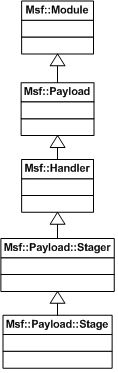
\includegraphics[height=4.0in]{dev_guide_payload_hierarchy}
\caption{Staged payload class hierarchy} \label{fig-img-payload}
\end{center}
\end{figure}

        \subsection{Interface}

\par
The framework uses a well-defined, uniform interface to work with
payload modules.  Like other modules, payload modules also have
module-specific information hash elements.  The table shown in
figure \ref{fig-table-payload-hash} shows the elements that are
specific to payload module information hash and the accessors that
can be used to access them.

\begin{figure}[h]
\begin{center}
\begin{tabular}{|l|l|l|p{2.0in}|}
\hline
\textbf{Hash Element} & \textbf{Accessor} & \textbf{Type} & \textbf{Description} \\
\hline
BadChars & badchars & String & The string of bad characters for this payload, if any. \\
\hline
SaveRegisters & save\_registers & Array & An array of architecture specific registers that should be saved when using this payload. \\
\hline
Payload & module\_info['Payload'] & Hash & A hash of information specific to this payload. \\
\hline
Convention & convention & String & The staging convention used by this payload, if any. \\
\hline
SymbolLookup & symbol\_lookup & String & The method used to resolved symbols by this payload, if any. \\
\hline
Handler & handler\_klass & Msf::Handler::Xxx & The handler class to be used with this payload, or \texttt{Msf::Handler::None}. \\
\hline
Session & session & Msf::Session::Xxx & The session class to create when the payload succeeds. \\
\hline
\end{tabular}
\caption{\texttt{Msf::Payload} information hash accessors}
\label{fig-table-payload-hash}
\end{center}
\end{figure}

\par
Using the payload-specific information, the framework drives the
payload class by using a specific set of methods.  These methods are
described in detail below.

            \subsubsection{compatible\_convention?}

\par
This method checks to see if the supplied staging convention is
compatible with the current payload module's staging convention.  If
the current payload's staging convention is undefined (as would be
the case for a non-staged payload) or the conventions match, then
true is returned.  Alternatively, if the current payload's type is
that of a stager and the supplied convention is undefined, then true
is also returned.  In every other case, false is returned.

            \subsubsection{compatible\_encoders}

\par
This method returns an array of compatible encoders where each
element in the array is an array with two elements that contains the
reference name of the encoder and the encoder's module class.

            \subsubsection{compatible\_nops}

\par
This method returns an array of compatible NOP generators where each
element in the array is an array with two elements that contains the
reference name of the NOP generator and the nop's module class.

            \subsubsection{connection\_type}

\par
This method returns the type of connection being used for this
payload as derived from the payload's handler.

            \subsubsection{generate}

\par
This method causes the underlying payload to be generated.  This
method works by calling the \texttt{payload} method on the payload
module instance and creating a duplicate copy of it.  From there,
any defined variables are substituted as conveyed through the
\texttt{offsets} attribute.  The resultant substituted buffer is
then returned to the caller.

            \subsubsection{payload\_type}

\par
This method returns the type of the payload that is implemented by
the derived class.  This can be one of
\texttt{Msf::Payload::Type::Single},
\texttt{Msf::Payload::Type::Stager}, or
\texttt{Msf::Payload::Type::Stage}.

            \subsubsection{size}

\par
This method returns the size of the payload as returned by a call to
\texttt{generate}.

            \subsubsection{staged?}

\par
This method returns true if the payload type is either
\texttt{Stager} or \texttt{Stage}.

            \subsubsection{substitute\_vars}

\par
This method substitutes variables using the \texttt{offsets} hash as
a guide.  It also calls \texttt{replace\_var} prior to doing
substitution which gives derived classes a chance to do custom
variable substitution prior to using built-in facilities.

            \subsubsection{validate}

\par
This method wraps the call to the payload's option container's
validate method.

        \subsection{Types}

\par
Framework payloads are broken down into three distinct payload
types.  The first type of payload that can be implemented is
referred to as a \textit{single} payload.  Single payloads are
self-contained, single stage payloads that do no undergo a staging
process.  An example of a typical single payload is one that
connects back to an attacker and supplies them with a shell without
any intermediate staging.  The second type of payload is referred to
as a \textit{stager}.  Stages are responsible for connecting back to
the attacker in some fashion and processing a second stage payload.
The third type of payload is referred to as a \textit{stage} and it
is what's executed by a stager payload.  These three payload types
allow the framework to dynamically generated various combinations of
payloads.

            \subsubsection{Single}

\par
As described above, single payloads are self-contained, single-stage
payloads that perform one logical task without requiring any
secondary code.  Single payloads are the simplest of the three
payload types because they correlate one-to-one with the payloads
that end up being generated by the framework.

\par
For single payloads, the module information hash's \texttt{Payload}
hash element will contain a sub-hash with a few key elements. The
table shown in figure \ref{fig-table-single-payload-hash} describes
the hash elements that are used by the framework and the accessors
that are used to obtain them.

\begin{figure}[h]
\begin{center}
\begin{tabular}{|l|l|l|p{2.0in}|}
\hline
\textbf{Hash Element} & \textbf{Accessor} & \textbf{Type} & \textbf{Description} \\
\hline
Payload & payload & String & The raw payload associated with this payload module. \\
\hline
Offsets & offsets & Hash & An array of variables that should be substituted at specific offsets based on the module's datastore. \\
\hline
\end{tabular}
\caption{Payload information sub-hash accessors}
\label{fig-table-single-payload-hash}
\end{center}
\end{figure}

\par
For single payloads, the \texttt{Payload} hash typically contains a
\texttt{Payload} sub-hash element that actually contains the raw
payload.  This is illustrated below:

\begin{verbatim}
    {
        'Payload' =>
            {
                'Payload' => "\xcc\xcc\xcc",
                'Offsets' => ...
            }
    }
\end{verbatim}

            \subsubsection{Stage}

\par
A stage payload is an implementation of a connection-independent
task like spawning a command shell or running an arbitrary command.
Stage payloads are combined with various framework stagers to
produce a set of connection-oriented multi-stage payloads.  This is
done automatically by the framework by associating stage payloads
with stagers that have a compatible staging convention.  The staging
convention describes the manner in which connection information is
passed from the stager to the stage in terms of what register might
hold a file descriptor, for instance.  Stages and stagers are also
matched up by their symbol lookup convention if necessary so that
stages can assume that certain locations in memory will hold
routines that may be useful.

\par
Stage payloads convey their raw payload contents in relation to the
\texttt{Stage} module information hash element.  The sub-hash
elements are similar to the single-style payloads in that it has
both a \texttt{Payload} and an \texttt{Offsets} element.

\par
Stage payloads are meaningless unless there is a compatible stager.

            \subsubsection{Stager}

\par
A stager payload is an implementation of a payload that establishes
some communication channel with the attacker to read in or otherwise
obtain a second stage payload to execute.  For example, a stager
might connection back to the attacker on a defined port and read in
code to execute.

\par
Stagers convey their raw payload contents in relation to the
\texttt{Stager} module information hash element.  The sub-hash
elements are similar to single-style payloads in that it has both a
\texttt{Payload} and an \texttt{Offsets} element.

\par
Furthermore, staged payloads have some extra accessor methods that
single payloads do not.  For instance, the stager's payload and
offsets can be obtained through the \texttt{payload} and
\texttt{offsets} accessors.  The stage's payload and offsets can be
obtained through the \texttt{stage\_payload} and
\texttt{stage\_offsets} accessors.

\par
The code below shows how those hash elements would be set up:


\begin{verbatim}
    {
        'Stager' =>
            {
                'Payload' => "\xcc\xcc\xcc",
                'Offsets' => ...
            },
        'Stage' =>
            {
                'Payload' => "\xcc\xcc\xcc",
                'Offsets' => ...
            }
    }
\end{verbatim}

        \subsection{Handlers}

\par
Handles are one of the critical components of a payload.  They are
responsible for handling the attacker's half of establishing a
connection that might be created by the payload being transmitted
via an exploit.  The different handlers will be discussed in detail
later in this subsection.

\par
Handlers themselves act as mixins that get merged into an actual
payload module class.  The framework interacts with handlers through
a well-defined interface.  Prior to initiating an exploit, the
framework will call into the payload handler's
\texttt{setup\_handler} and \texttt{start\_handler} methods that
will lead to the initialization of the handler in preparation for a
payload connection.  When a connection arrives, the handler calls
the \texttt{handle\_connection} method on the payload instance. This
method is intended to be overridden as necessary by the payload to
do custom tasks.  For instance, staged payloads will initiate the
transfer of the second stage over the established connection and
then call the default implementation which leads to the creation of
a session for the connection.

\par
When an exploit has finished, the framework will call into the
payload handlers \texttt{stop\_handler} and
\texttt{cleanup\_handler} methods to stop it from listening for
future connections.

            \subsubsection{Bind TCP}

\par
The bind TCP handler is provided through
\texttt{Msf::Handler::BindTcp}.  It will attempt to establish a
connection to a target machine on a given port (specified in
\texttt{LPORT}).  If a connection is established, a call is made
into \texttt{handle\_connection} passing along the socket associated
with the connection.

            \subsubsection{Find port}

\par
The find port handler is provided by the
\texttt{Msf::Handler::FindPort} class.  When an exploit calls the
\texttt{handler} method with a socket connection, the find port
handler will attempt to see if the socket has now been re-purposed
for use by the payload.  The find port handler is meant to be used
for payloads that search for a socket by comparing peer port names
relative to the target machine.

            \subsubsection{Find tag}

\par
The find port handler is provided by the
\texttt{Msf::Handler::FindTag} class.  When an exploit calls the
\texttt{handler} method with a socket connection, the find port
handler will attempt to see if the socket has now been re-purposed
for use by the payload.  The find tag handler is meant to be used
for find socket style payloads that search for a socket based on the
presence of a tag on the wire.

            \subsubsection{None}

\par
If a payload does not establish a connection of any sort, the
\texttt{Msf::Handler::None} handler is used.

            \subsubsection{Reverse TCP}

\par
The reverse TCP handler is provided by the
\texttt{Msf::Handler::ReverseTcp} class.  It will listen on a port
for incoming connections and will make a call into
\texttt{handle\_connection} with the client sockets as they do.

    \section{Recon}

\par
The reconnaissance module is still undergoing design review and will
not be documented at this time.

\chapter{Framework Plugins}
\label{framework-plugins}

\par
The 3.0 version of the framework offers a new type of framework
concept which is that of the \textit{framework plugin}.  Unlike
modules, framework plugins are designed to alter or augment the
framework itself.  The scope under which plugins fall is
intentionally very broad as to encourage free flowing creativity
with what they might be capable of doing.  The interface for a
plugin is intentionally very simple.  All plugins must exist under
the \texttt{Msf::Plugin} namespace and they must inherit the
\texttt{Msf::Plugin} base class.  Plugins are loaded into the
framework by calling \texttt{framework.plugins.load} with a file
path that contains the plugin.  The framework will then take care of
loading the plugin and creating an instance of the class found
within the file specified, assuming the class was added to the
\texttt{Msf::Plugin} namespace.

\par
When the framework creates an instance of a plugin, it calls the
plugin's constructor and passes it the framework instance that it's
being created from.  It also passes along a hash of arbitrary
parameters, some of which have a well-defined purpose as described
in the chapter on the plugin manager in the framework core
documentation.  Alternatively, a plugin could be passed custom
initialization parameters through the options hash.

\par
To understand the types of things a framework plugin is capable of,
a few different theoretical examples will be enumerated in this
chapter.  The first example would be a plugin that simply adds a new
command to the console interface when loaded that performs some
simple task.  The sample plugin included with the default
distribution of the framework illustrates how this can be
accomplished.  A more advanced plugin might automate some of the
actions taken when a Meterpreter session is created, such as by
automatically downloading the remote machine's password hashes and
passing them off to a cracking program.

\par
Another example of a plugin would be introducing an entirely new
module type into the framework.  This would be accomplished by
extending the existing framework instance to support accessors for
dealing with the new module type.

\chapter{Framework Sessions}
\label{framework-sessions}

\par
The typical end-game for an exploit is to provide the attacker with
some type of session that allows them to run commands or perform
other actions on a target machine.  In most cases, this session is a
typical command interpreter that has had its input and output piped
over a socket connection to the attacker.  However, a command shell
in and of itself is no particularly automatable unless wrapped in a
class that allows access to the shell from the level of a command
script.  It is for this reason that the 3.0 version of the framework
emphasizes generalized session classes that can be used by the
framework, plugins, and external scripts to automate the process of
controlling a session that is created after an exploit succeeds.

\par
To provide an extensible level of automation control, framework
sessions can implement one or more of the provider mixins found
under the \texttt{Msf::Session::Provider} namespace.  The current
distribution of the framework provides four basic provider
interfaces that can be implemented by specific sessions.

\begin{enumerate}
    \item \texttt{MultiCommandExecution}

This interface provides methods that can be used to execute
multiple simultaneous  commands on the target machine.  This
interface is a super-set of the \texttt{SingleCommandExecution}
interface.

    \item \texttt{MultiCommandShell}

This interface provides methods for executing multiple command
shells simultaneously on the target machine.  This interface is a
super-set of the \texttt{SingleCommandShell} interface.

    \item \texttt{SingleCommandExecution}

This interface provides methods for executing a single command on
the target machine.

    \item \texttt{SingleCommandShell}

This interface provides methods for executing a single command shell
on the target machine.

\end{enumerate}

\par
By implementing one or more of these methods, sessions can be made
programmatically automatable at the most basic level.  Aside from
the standard interfaces, sessions can also optionally implement the
\texttt{Msf::Session::Comm} mixin which is intended to be used for
channeling network traffic through a remote machine.  Sessions that
implement the \texttt{Msf::Session::Comm} mixin can be used in
conjunction with the switch board routing table present in the Rex
library.

\par
At the time of this writing, there are two basic session
implementations that are found in the framework base library.  These
two sessions are described in the following sections.

    \section{Command Shell}

\par
The command shell session provided through
\texttt{Msf::Sessions::CommandShell} implements the
\texttt{Msf::Session::Provider::SingleCommandShell} interface.  The
methods used to interact with the shell are simply tunneled over the
stream associated with the remote side of the connection.  Any
payload that renders a command shell should return an instance of
this session.

    \section{Meterpreter}

\par
The meterpreter session provided through
\texttt{Msf::Sessions::Meterpreter} implements the
\texttt{Msf::Session::Comm} interface and is also capable of
implementing some of the other automated interfaces.  By
implementing the Comm interface, all meterpreter sessions can be
used for pivoting network traffic.

\chapter{Methodologies}

\par
One of the most critical things to understand prior to attempting to
write a module for the framework are some of the methodologies that
should be undertaken.  The goal of the 3.0 version of the framework
is to make modules easier to implement and at the same time make
them more robust.  With that goal in mind, all programmers wishing
to write framework modules should heed the advice from this chapter.

\par
First and foremost, modules should be simple.  In the event that a
module is becoming complicated or large, it may be best to take a
step back and see if any of the code being put into it might be
better generalized in a mixin that could later be shared with other
modules.  This is especially true in the event that an exploit is
dealing with a protocol that may later be useful to other exploits.
An equally true case is when an exploit is attempting to trigger a
vulnerability that has a generalized approach that could be applied
to other exploit modules.

\par
Secondly, modules should be clean.  One of the key factors when
doing any sort of development is to ensure consistency in both
design and implementation.  This applies not only to naming schemes
but also to things like indention.  If a module has inconsistent
indention and/or naming schemes, its readability will be drastically
reduced.  Every programmer is entitled to their own coding style,
but they should be sure to stick with it throughout the development
of a given unit.

\par
Finally, encapsulation is king.  If a module needs to perform an
action that could perhaps be changed to a different algorithm at a
later date, encapsulating the operation in a generalized interface
is a great way to ensure that code does not have to be rewritten or
otherwise altered in the future.

\appendix
\chapter{Samples}

\par
This chapter contains various samples that illustrate how the
framework and other libraries can be interacted with to perform
various tasks.  The source code to these samples can be found in the
documentation directory that is included with all releases of the
3.0 version of the framework.

    \section{Framework}

\par
This section contains samples specific to interacting with the
framework itself.

        \subsection{Dumping module info}

\par
This sample demonstrates how a module's information can be easily
serialized to a readable format.

\footnotesize{
\begin{verbatim}
#!/usr/bin/ruby

$:.unshift(File.join(File.dirname(__FILE__), '..', '..', '..',
   'lib'))

require 'msf/base'

if (ARGV.empty?)
   puts "Usage: #{File.basename(__FILE__)} module_name"
   exit
end

framework = Msf::Simple::Framework.create

begin
   # Create the module instance.
   mod = framework.modules.create(ARGV.shift)

   # Dump the module's information in readable text format.
   puts Msf::Serializer::ReadableText.dump_module(mod)
rescue
   puts "Error: #{$!}\n\n#{$@.join("\n")}"
end
\end{verbatim}}

        \subsection{Encoding the contents of a file}

\par
This sample demonstrates how a file can be encoded using a framework
encoder.

\footnotesize{
\begin{verbatim}
#!/usr/bin/ruby

$:.unshift(File.join(File.dirname(__FILE__), '..', '..', '..',
   'lib'))

require 'msf/base'

if (ARGV.empty?)
   puts "Usage: #{File.basename(__FILE__)} encoder_name file_name format"
   exit
end

framework = Msf::Simple::Framework.create

begin
   # Create the encoder instance.
   mod = framework.encoders.create(ARGV.shift)

   puts(Msf::Simple::Buffer.transform(
      mod.encode(IO.readlines(ARGV.shift).join), ARGV.shift || 'ruby'))
rescue
   puts "Error: #{$!}\n\n#{$@.join("\n")}"
end
\end{verbatim}}

        \subsection{Enumerating modules}

\par
This sample demonstrates enumerating all of the modules in the
framework and displays their module type and reference name.

\footnotesize{
\begin{verbatim}
#!/usr/bin/ruby

$:.unshift(File.join(File.dirname(__FILE__), '..', '..', '..',
  'lib'))

require 'msf/base'

framework = Msf::Simple::Framework.create

# Enumerate each module in the framework.
framework.modules.each_module { |name, mod|
   puts "#{mod.type}: #{name}"
}
\end{verbatim}}

        \subsection{Running an exploit using framework base}

\par
This sample demonstrates using the framework core directly to
launch an exploit.  It makes use of the simplified exploit wrapper
method provided by the Msf::Simple::Exploit mixin.

\footnotesize{
\begin{verbatim}
#!/usr/bin/ruby

$:.unshift(File.join(File.dirname(__FILE__), '..', '..', '..',
   'lib'))

require 'msf/base'

if (ARGV.length == 0)
   puts "Usage: #{File.basename(__FILE__)} exploit_name payload_name OPTIONS"
   exit
end

framework    = Msf::Simple::Framework.create
exploit_name = ARGV.shift || 'test/multi/aggressive'
payload_name = ARGV.shift || 'windows/meterpreter/reverse_tcp'
input        = Rex::Ui::Text::Input::Stdio.new
output       = Rex::Ui::Text::Output::Stdio.new

begin
   # Initialize the exploit instance
   exploit = framework.exploits.create(exploit_name)

   # Fire it off.
   session = exploit.exploit_simple(
      'Payload'     => payload_name,
      'OptionStr'   => ARGV.join(' '),
      'LocalInput'  => input,
      'LocalOutput' => output)

   # If a session came back, try to interact with it.
   if (session)
      output.print_status("Session #{session.sid} created, interacting...")
      output.print_line

      session.init_ui(input, output)

      session.interact
   else
      output.print_line("Exploit completed, no session was created.")
   end

rescue
   output.print_error("Error: #{$!}\n\n#{$@.join("\n")}")
end
\end{verbatim}}


        \subsection{Running an exploit using framework core}

\par
This sample demonstrates using the framework core directly to launch
an exploit.  It uses the framework base Framework class so that the
distribution module path is automatically set, but relies strictly
on framework core classes for everything else.

\footnotesize{
\begin{verbatim}
#!/usr/bin/ruby

$:.unshift(File.join(File.dirname(__FILE__), '..', '..', '..',
   'lib'))

require 'msf/base'

if (ARGV.length == 0)
   puts "Usage: #{File.basename(__FILE__)} exploit_name payload_name OPTIONS"
   exit
end

framework    = Msf::Simple::Framework.create
exploit_name = ARGV.shift || 'test/multi/aggressive'
payload_name = ARGV.shift || 'windows/meterpreter/reverse_tcp'
input        = Rex::Ui::Text::Input::Stdio.new
output       = Rex::Ui::Text::Output::Stdio.new

begin
   # Create the exploit driver instance.
   driver = Msf::ExploitDriver.new(framework)

   # Initialize the exploit driver's exploit and payload instance
   driver.exploit = framework.exploits.create(exploit_name)
   driver.payload = framework.payloads.create(payload_name)

   # Import options specified in VAR=VAL format from the supplied command
   # line.
   driver.exploit.datastore.import_options_from_s(ARGV.join(' '))

   # Share the exploit's datastore with the payload.
   driver.payload.share_datastore(driver.exploit.datastore)

   # Initialize the target index to what's in the exploit's data store or
   # zero by default.
   driver.target_idx = (driver.exploit.datastore['TARGET'] || 0).to_i

   # Initialize the exploit and payload user interfaces.
   driver.exploit.init_ui(input, output)
   driver.payload.init_ui(input, output)

   # Fire it off.
   session = driver.run

   # If a session came back, try to interact with it.
   if (session)
      output.print_status("Session #{session.sid} created, interacting...")
      output.print_line

      session.init_ui(input, output)

      session.interact
   else
      output.print_line("Exploit completed, no session was created.")
   end

rescue
   output.print_error("Error: #{$!}\n\n#{$@.join("\n")}")
end
\end{verbatim}}

    \section{Framework Module}

\par
This section shows some sample framework modules.

        \subsection{Encoder}

\par
This sample illustrates a very basic encoder that simply returns the
block that it's passed.

\footnotesize{
\begin{verbatim}
module Msf
module Encoders

class Sample < Msf::Encoder

   def initialize
      super(
         'Name'             => 'Sample encoder',
         'Version'          => '$Revision$',
         'Description'      => %q{
            Sample encoder that just returns the block it's passed
            when encoding occurs.
         },
         'Author'           => 'skape',
         'Arch'             => ARCH_ALL)
   end

   #
   # Returns the unmodified buffer to the caller.
   #
   def encode_block(state, buf)
      buf
   end

end

end
end
\end{verbatim}}

        \subsection{Exploit}

\par
This exploit sample shows how an exploit module could be written to
exploit a bug in an arbitrary TCP server.

\footnotesize{
\begin{verbatim}
module Msf

class Exploits::Sample < Msf::Exploit::Remote

   #
   # This exploit affects TCP servers, so we use the TCP client mixin.
   #
   include Exploit::Remote::Tcp

   def initialize(info = {})
      super(update_info(info,
         'Name'           => 'Sample exploit',
         'Description'    => %q{
            This exploit module illustrates how a vulnerability could be exploited
            in an TCP server that has a parsing bug.
         },
         'Author'         => 'skape',
         'Version'        => '$Revision$',
         'Payload'        =>
            {
               'Space'    => 1000,
               'BadChars' => "\x00",
            },
         'Targets'        =>
            [
               # Target 0: Windows All
               [
                  'Windows Universal',
                  {
                     'Platform' => 'win',
                     'Ret'      => 0x41424344
                  }
               ],
            ],
         'DefaultTarget' => 0))
   end

   #
   # The sample exploit just indicates that the remote host is always
   # vulnerable.
   #
   def check
      return Exploit::CheckCode::Vulnerable
   end

   #
   # The exploit method connects to the remote service and sends 1024 A's
   # followed by the fake return address and then the payload.
   #
   def exploit
      connect

      print_status("Sending #{payload.encoded.length} byte payload...")

      # Build the buffer for transmission
      buf  = "A" * 1024
      buf += [ target.ret ].pack('V')
      buf += payload.encoded

      # Send it off
      sock.put(buf)
      sock.get

      handler
   end

end

end
\end{verbatim}}

        \subsection{Nop}

\par
This class implements a very basic NOP sled generator that just
returns a string of 0x90's for the supplied sled length.

\footnotesize{
\begin{verbatim}
module Msf
module Nops

class Sample < Msf::Nop

   def initialize
      super(
         'Name'        => 'Sample NOP generator',
         'Version'     => '$Revision$',
         'Description' => 'Sample single-byte NOP generator',
         'Author'      => 'skape',
         'Arch'        => ARCH_X86)
   end

   #
   # Returns a string of 0x90's for the supplied length.
   #
   def generate_sled(length, opts)
      "\x90" * length
   end

end

end
end
\end{verbatim}}

        \subsection{Payload}

\par
This sample payload is designed to trigger a debugger exception via
int3.

\footnotesize{
\begin{verbatim}
module Msf
module Payloads
module Singles

module Sample

   include Msf::Payload::Single

   def initialize(info = {})
      super(update_info(info,
         'Name'          => 'Debugger Trap',
         'Version'       => '$Revision$',
         'Description'   => 'Causes a debugger trap exception through int3',
         'Author'        => 'skape',
         'Platform'      => 'win',
         'Arch'          => ARCH_X86,
         'Payload'       =>
            {
               'Payload' => "\xcc"
            }
         ))
   end

end

end
end
end
\end{verbatim}}

        \subsection{Recon}

\par
Reconnaissance modules are undergoing design review and do not have
any samples available at this time.

    \section{Framework Plugin}

        \subsection{Console user interface plugin}

\par
This class illustrates a sample plugin.  Plugins can change the
behavior of the framework by adding new features, new user interface
commands, or through any other arbitrary means.  They are designed
to have a very loose definition in order to make them as useful as
possible.

\footnotesize{
\begin{verbatim}
module Msf

class Plugin::Sample < Msf::Plugin

   ###
   #
   # This class implements a sample console command dispatcher.
   #
   ###
   class ConsoleCommandDispatcher
      include Msf::Ui::Console::CommandDispatcher

      #
      # The dispatcher's name.
      #
      def name
         "Sample"
      end

      #
      # Returns the hash of commands supported by this dispatcher.
      #
      def commands
         {
            "sample" => "A sample command added by the sample plugin"
         }
      end

      #
      # This method handles the sample command.
      #
      def cmd_sample(*args)
         print_line("You passed: #{args.join(' ')}")
      end
   end

   #
   # The constructor is called when an instance of the plugin is created.  The
   # framework instance that the plugin is being associated with is passed in
   # the framework parameter.  Plugins should call the parent constructor when
   # inheriting from Msf::Plugin to ensure that the framework attribute on
   # their instance gets set.
   #
   def initialize(framework, opts)
      super

      # If this plugin is being loaded in the context of a console application
      # that uses the framework's console user interface driver, register
      # console dispatcher commands.
      add_console_dispatcher(ConsoleCommandDispatcher)

      print_status("Sample plugin loaded.")
   end

   #
   # The cleanup routine for plugins gives them a chance to undo any actions
   # they may have done to the framework.  For instance, if a console
   # dispatcher was added, then it should be removed in the cleanup routine.
   #
   def cleanup
      # If we had previously registered a console dispatcher with the console,
      # deregister it now.
      remove_console_dispatcher('Sample')
   end

   #
   # This method returns a short, friendly name for the plugin.
   #
   def name
      "sample"
   end

   #
   # This method returns a brief description of the plugin.  It should be no
   # more than 60 characters, but there are no hard limits.
   #
   def desc
      "Demonstrates using framework plugins"
   end

end
end
\end{verbatim}

\end{document}
